

\begin{figure}[H]
    \caption{Progresa Enrollment Intensity and Mortality Rate Trends}
    \label{af:variation_all}

    {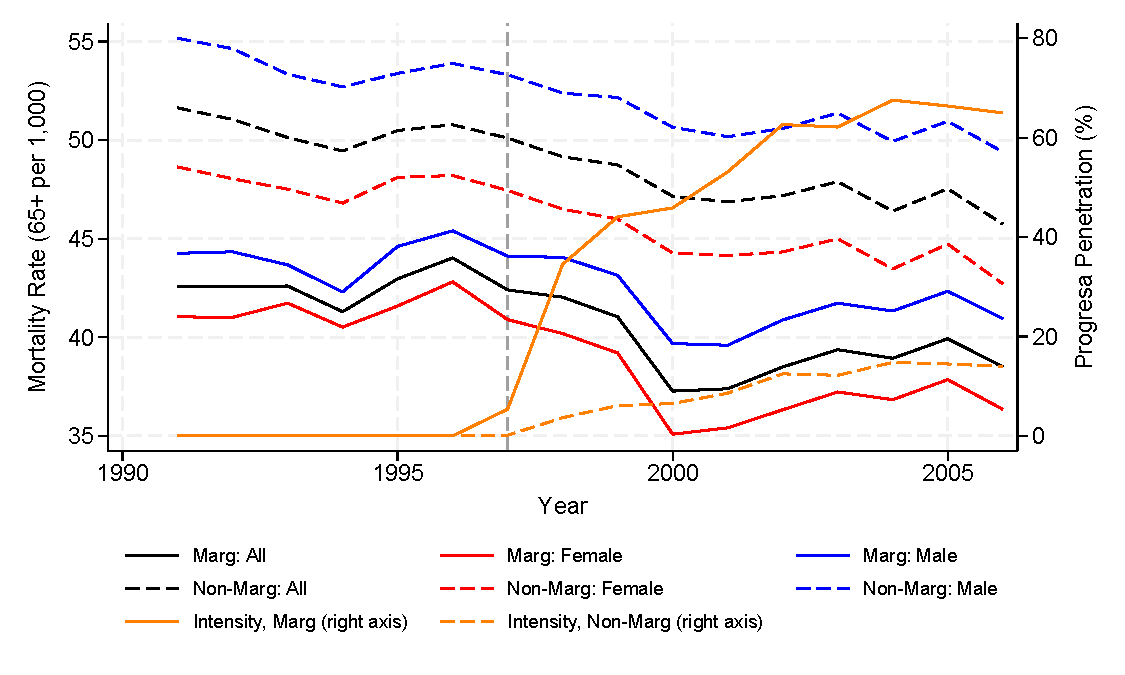
\includegraphics[width=0.89\textwidth]{figures/appendix/AF1_all.pdf}}

         \floatfoot{Notes: This figure documents trends variation in Progresa enrollment and mortality rates for older adults across all Mexican municipalities over 1991--2006. Highly marginalized municipalities are those classified as high or very high on the 1990 CONAPO Marginalization Index \citep{CONAPO1993}, constructed from nine census-based indicators capturing educational attainment, housing conditions and access to basic services, low income, and residence in small localities; non-marginalized municipalities are the three remaining levels.}
\end{figure}

\begin{figure}[H]
    \caption{Progresa Enrollment Intensity by Municipality Sample}
    \label{af:variation_maps}

    \subfigure[Intensity in 1999 - All]
     {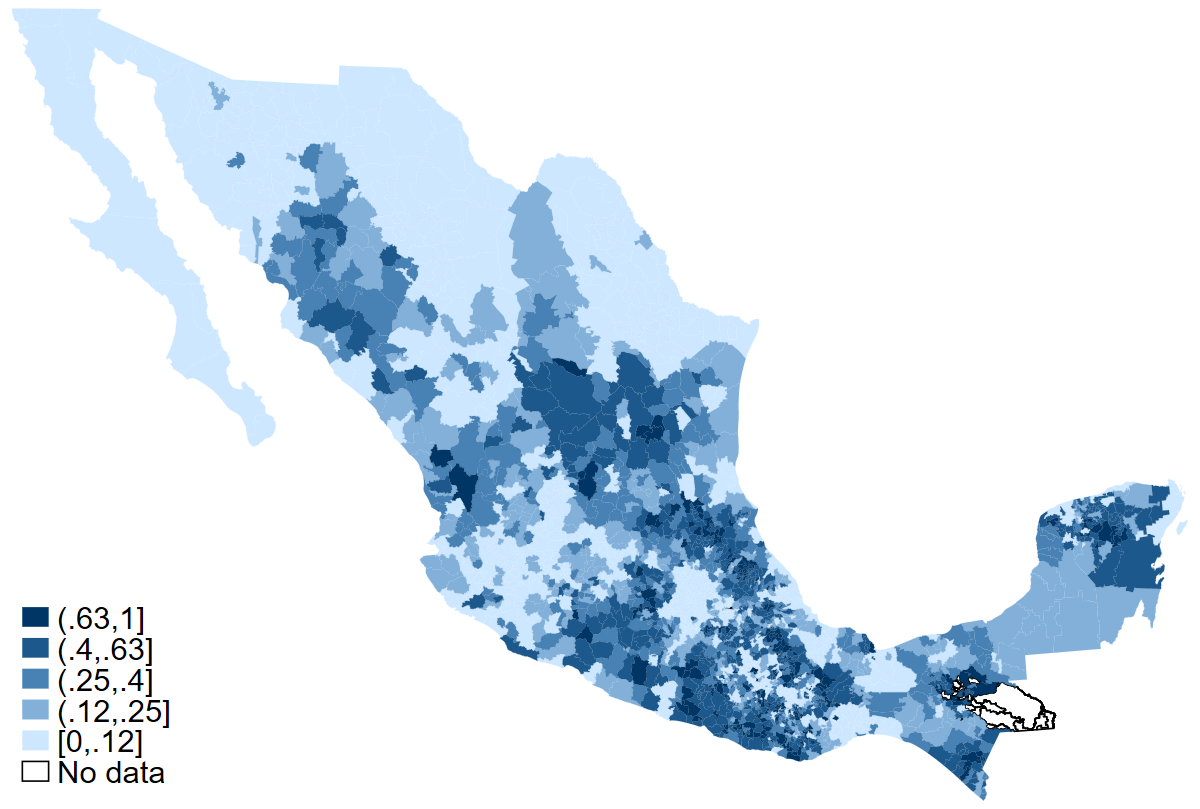
\includegraphics[width=0.49\textwidth]{figures/appendix/AF2a_inten1999_all.png}}
    \subfigure[Intensity in 2005 - All]
     {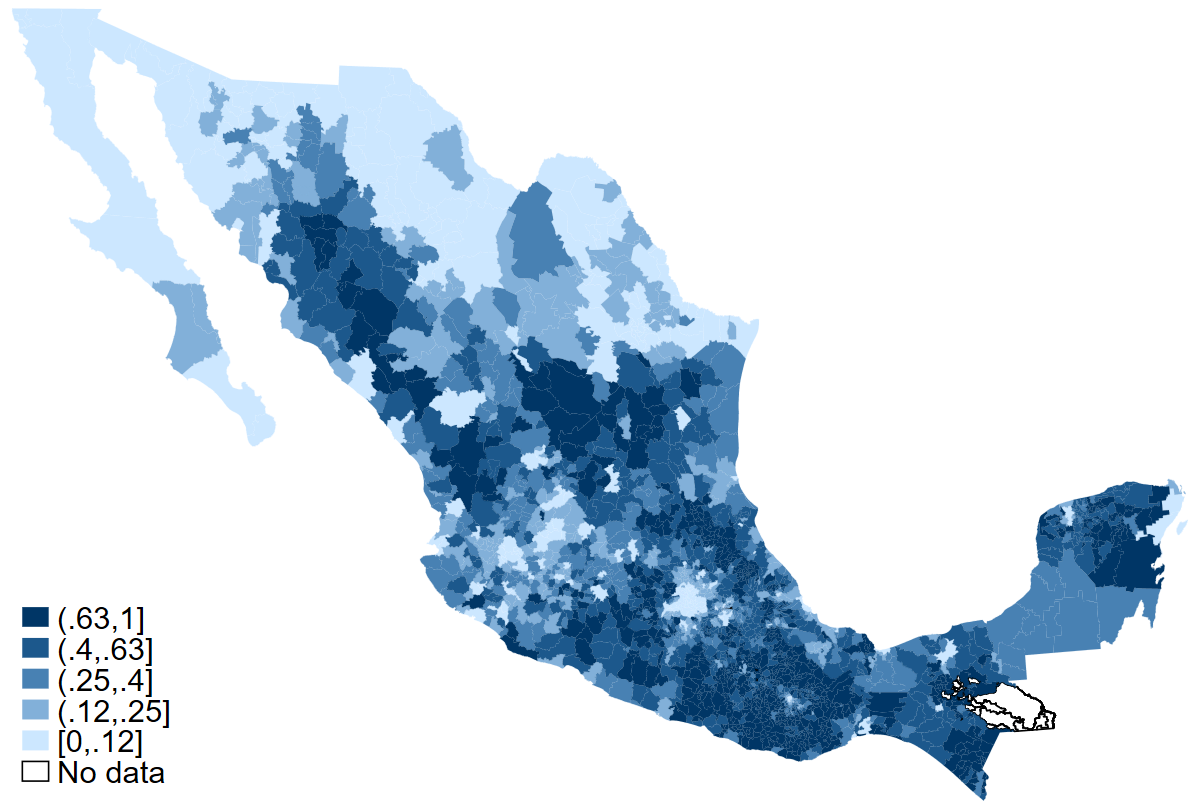
\includegraphics[width=0.49\textwidth]{figures/appendix/AF2b_inten2005_all.png}}
      \subfigure[Intensity in 1997 - Highly Marginalized]
     {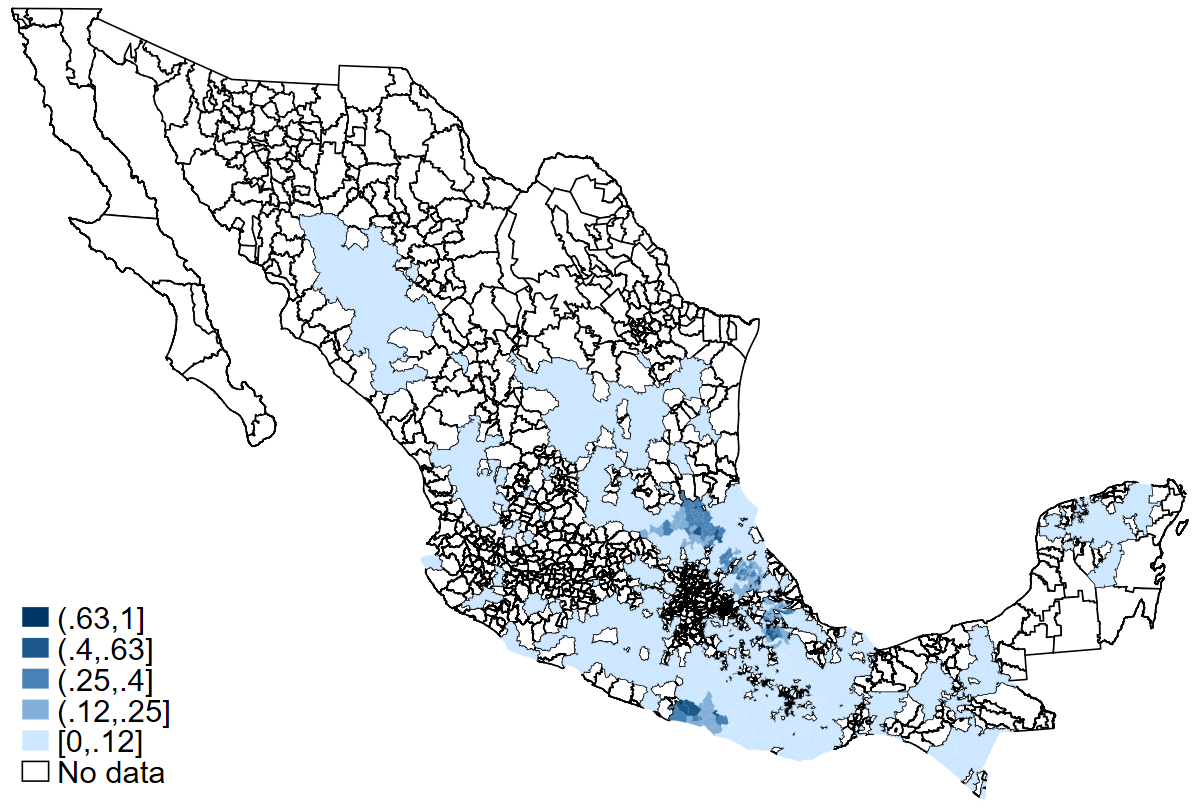
\includegraphics[width=0.49\textwidth]{figures/appendix/AF2c_inten1997_mort.png}}
    \subfigure[Intensity in 1997 - All]
     {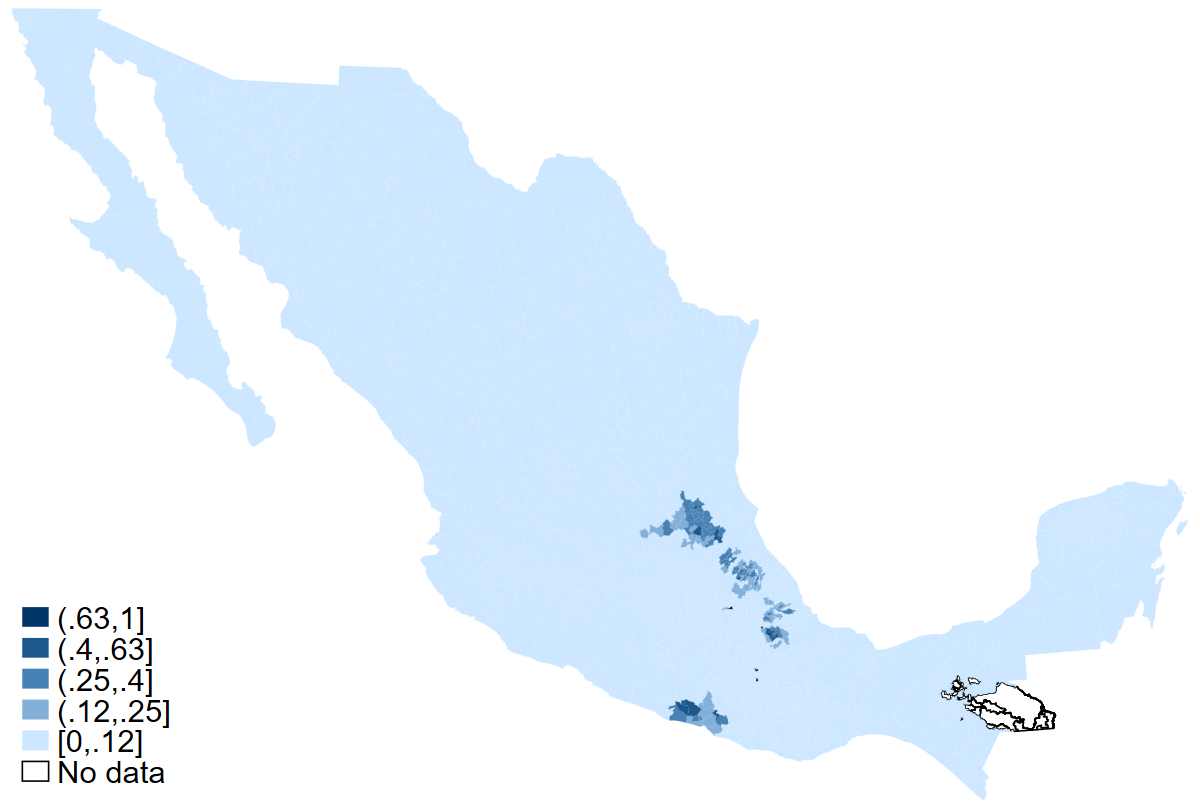
\includegraphics[width=0.49\textwidth]{figures/appendix/AF2d_inten1997_mort_all.png}}

         \floatfoot{Notes: This figure documents geographic variation in Progresa enrollment for all municipalities, complementing Figure~1 in the main text which focuses on the highly marginalized subsample. Panel~(a) and (b) map Progresa intensity across all municipalities for 1999 and 2005; panels~(c) and (d) map intensity in 1997 separately for highly marginalized municipalities (the main sample) and all municipalities. Darker shading indicates higher program intensity.}
\end{figure}

\begin{figure}[H]
    \caption{Progresa Enrollment Ratio by Roll-Out Phase and Marginality Percentile: Locality vs.\ Municipality}
    \label{af:enroll_loc_mun}

\subfigure[Locality level]
{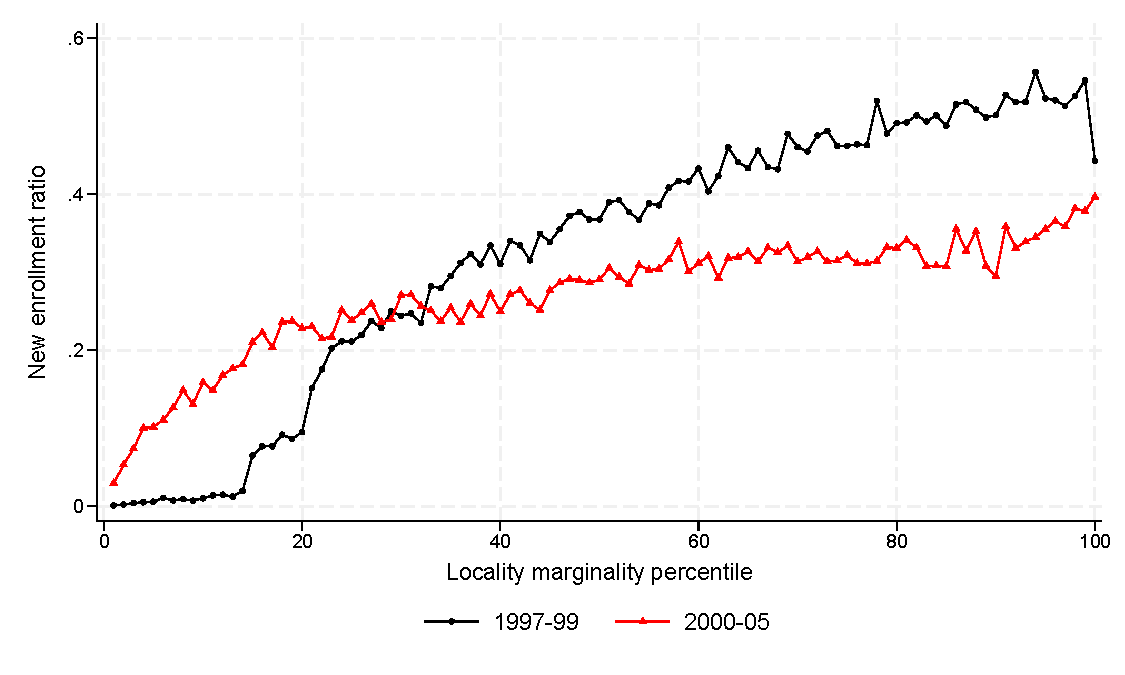
\includegraphics[width=0.7\textwidth]{figures/appendix/AF3a_enroll_loc_marg_pctile.pdf}}

\subfigure[Municipality level]
{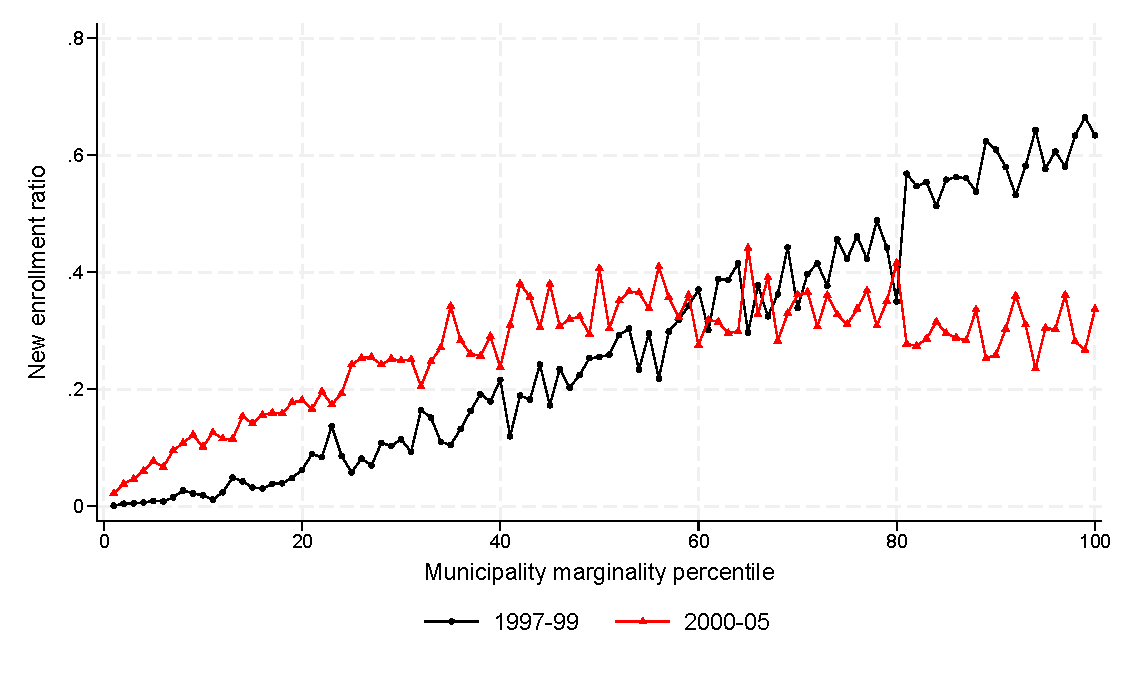
\includegraphics[width=0.7\textwidth]{figures/appendix/AF3b_enroll_mun_marg_pctile.pdf}}

         \floatfoot{Notes: This figure shows the enrollment ratio across the marginality percentile at the locality and municipality level. The horizontal axis is a percentile rank in the national distribution of the 1995 (locality) or 1990 (municipality) CONAPO marginalization index; each point is the mean new-enrollment ratio within a 1-point percentile bin. The black series is the early phase (1997--1999); the red series is the incremental enrollment added during the later phase (2000--2005). Both panels use all Mexican localities/municipalities (not only the highly marginalized subsample) to display the full national targeting gradient.}
\end{figure}


% NOTE: the cause-of-death event-study figures (former Appendix Figures
% AF4/AF5, af:es_cod_marg_a/af:es_cod_marg_b) have moved to
% codes/04_extra_robustness.do per the coauthor's request -- no longer
% displayed in the paper.


\begin{figure}[H]
    \caption{Event Study: Effect of Progresa Enrollment Intensity on Older Adults' Mortality Rate by Sex and SES-Trend Specification}
    \label{af:ses_trend}

\subfigure[Pooled]
{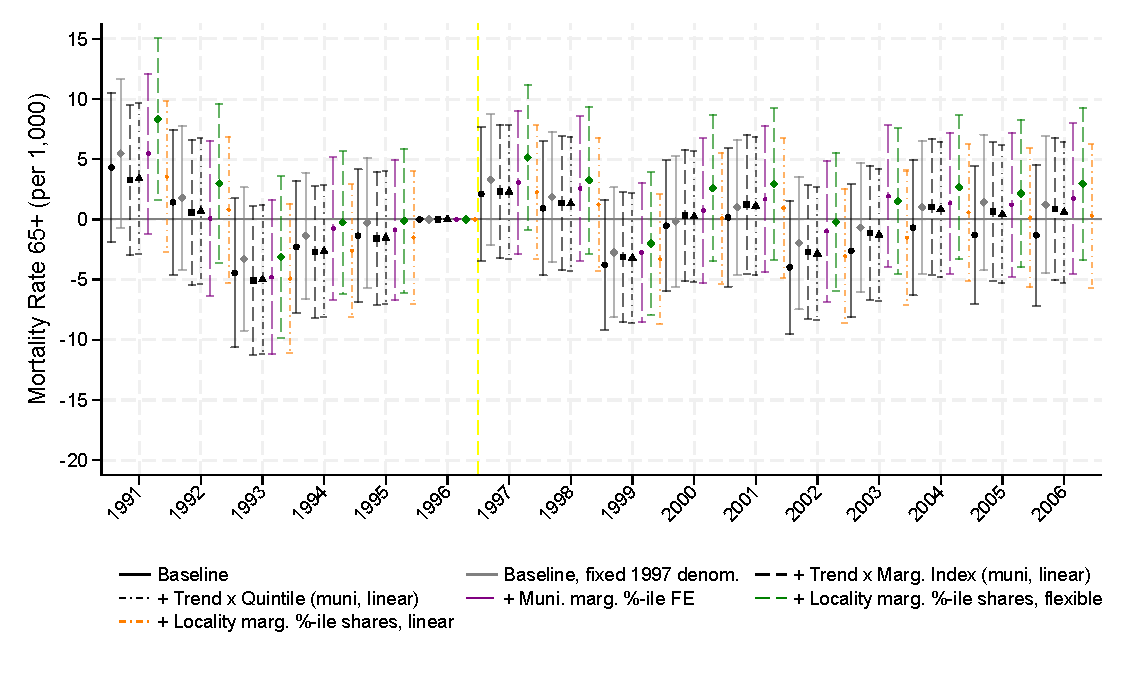
\includegraphics[width=0.65\textwidth]{figures/appendix/AF7a_ses_trend.pdf}}

\subfigure[Female]
{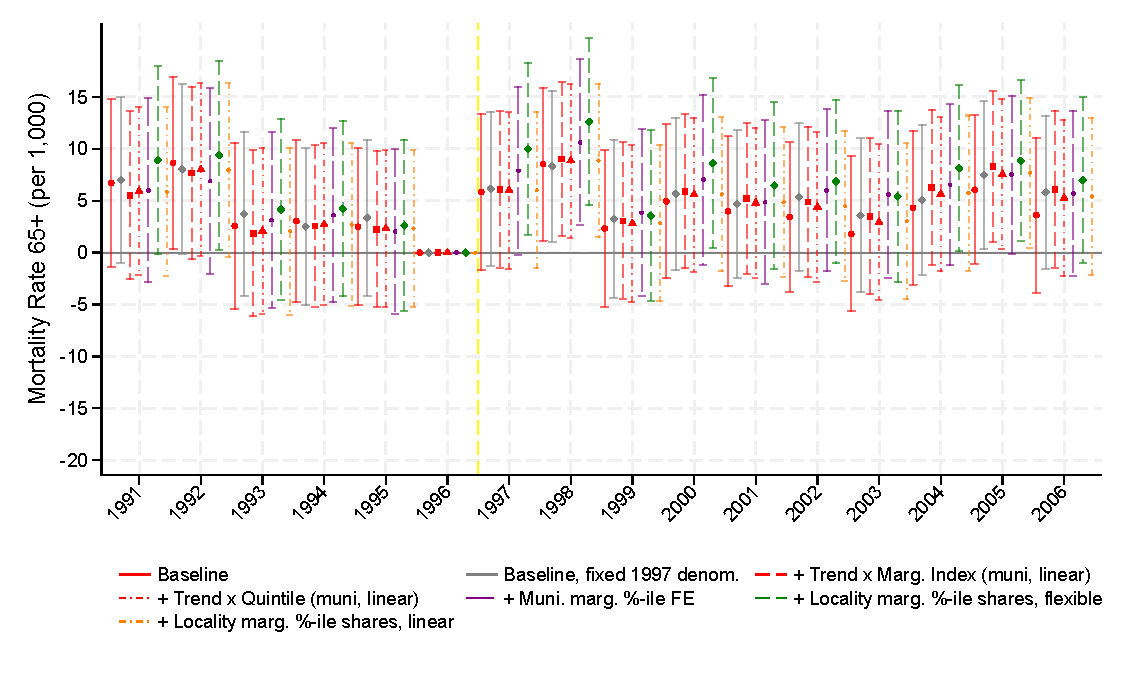
\includegraphics[width=0.49\textwidth]{figures/appendix/AF7b_ses_trend_f.pdf}}
\subfigure[Male]
{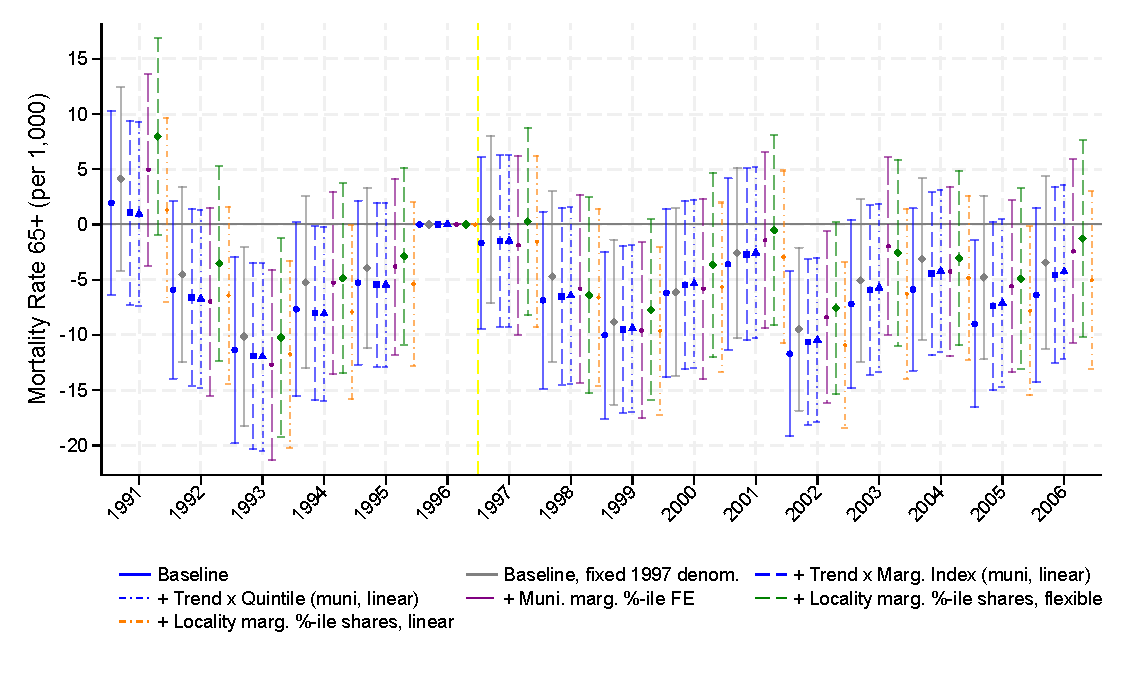
\includegraphics[width=0.49\textwidth]{figures/appendix/AF7c_ses_trend_m.pdf}}


         \floatfoot{Notes: Panels~(a)--(c) present event-study estimates of the interaction between $\textit{Intensity}_{1999}$ and year indicators (reference year 1996) for the pooled, female, and male older-adult (65+) mortality rate per 1,000 inhabitants, respectively. Within each panel, seven specifications are overlaid: (i) the baseline specifications; (i-b) the same baseline but with fixed 1997 household denominator; (ii) the baseline plus a municipality-specific linear time trend interacted with the continuous 1990 municipality marginalization index; (iii) the baseline plus a linear trend interacted with 1990 municipality marginalization-index quintiles; (iv) the baseline plus a full set of percentile-bin indicators of the marginalization index (100 bins); (v) the baseline plus a locality-marginality percentile-share control -- the share of each municipality's population residing in localities at each percentile of the national \textit{locality}-marginality distribution (five bins) -- interacted with a fully flexible set of year indicators; and (vi) the same locality-marginality percentile-share control interacted with a \emph{linear} year trend. All seven specifications control for $\textit{Intensity}_{2005}$ interaction. The vertical line marks the program's 1997 roll-out. The sample is restricted to highly marginalized municipalities and regressions are weighted by the population aged 65 and older. 95\% confidence intervals shown.}
\end{figure}


\begin{figure}[H]
    \caption{Event Study: Effect of Progresa Enrollment Intensity on Mortality Rate by Sex and Functional Forms}
    \label{af:es_func_form}

\subfigure[Levels - Weighted]
{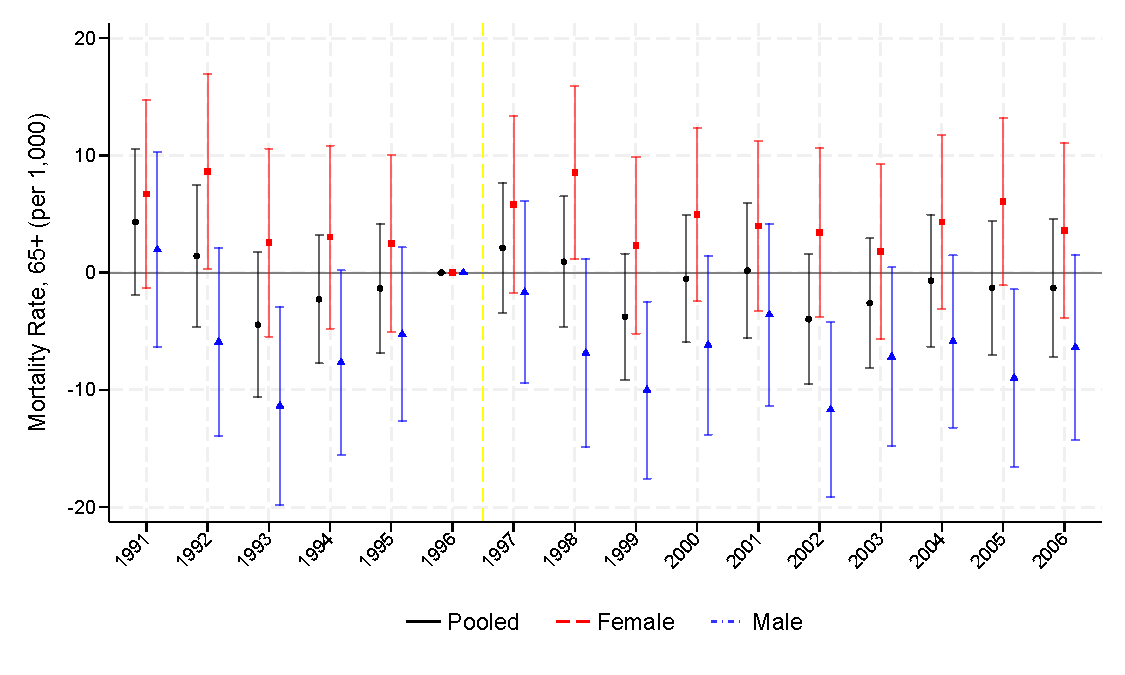
\includegraphics[width=0.49\textwidth]{figures/appendix/AF6a_ES_func_form_levels.pdf}}
  \subfigure[Levels - Unweighted]
{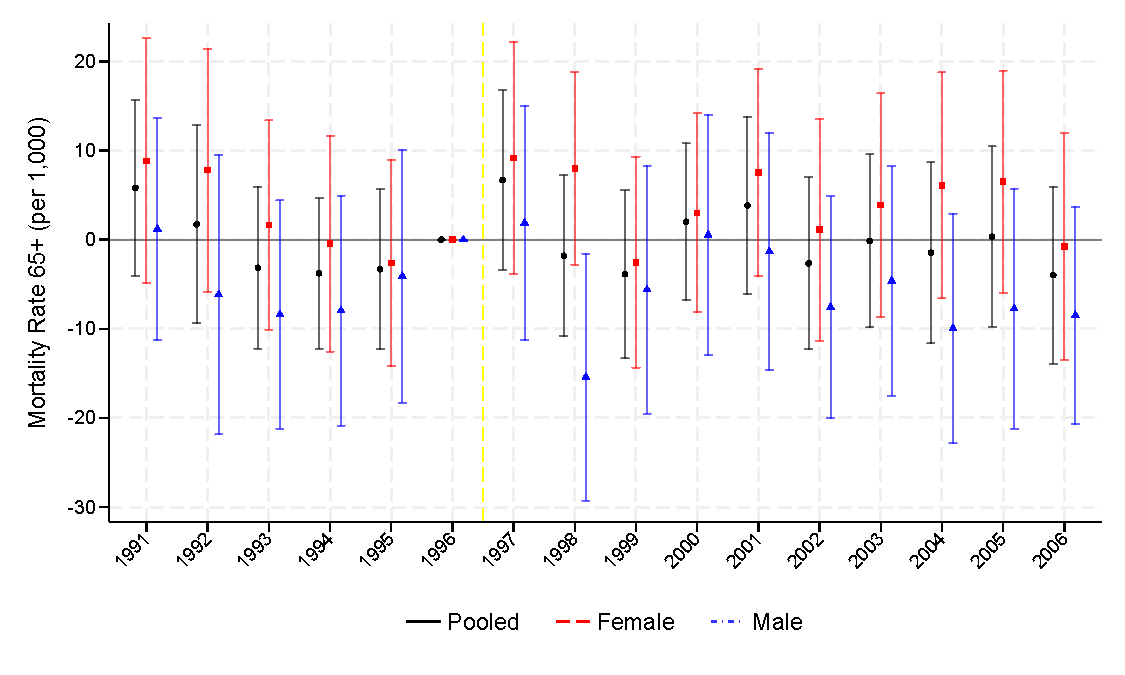
\includegraphics[width=0.49\textwidth]{figures/appendix/AF6b_uw.pdf}}


\subfigure[Logarithm]
{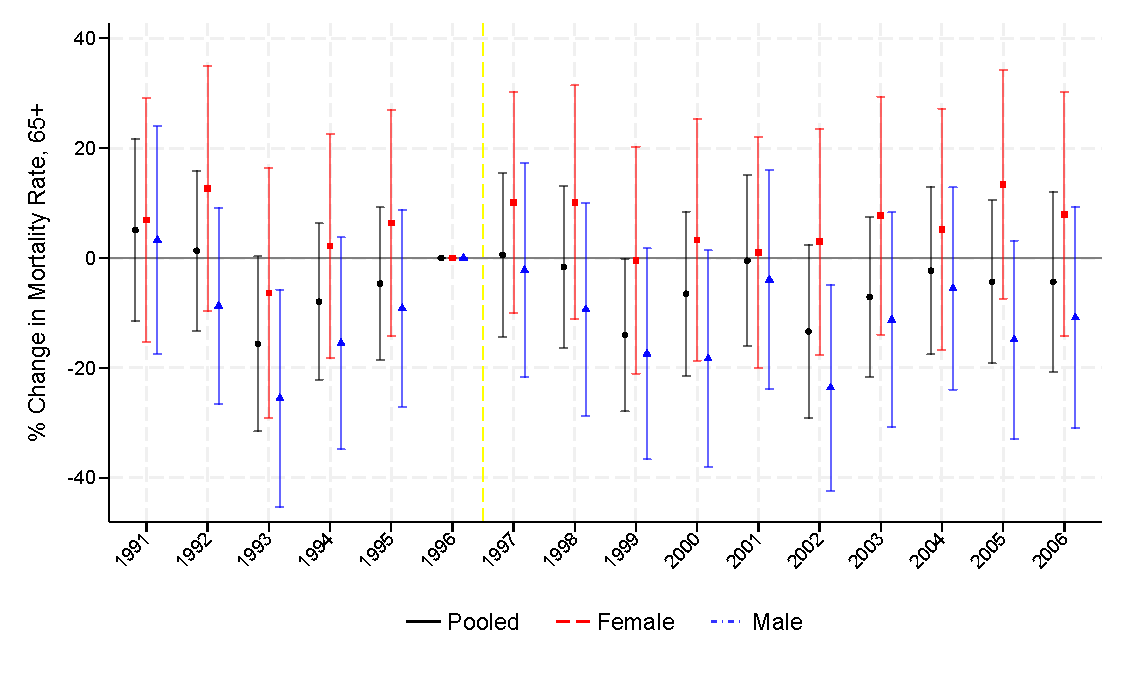
\includegraphics[width=0.49\textwidth]{figures/appendix/AF6c_ES_func_form_log.pdf}}
\subfigure[Poisson]
     {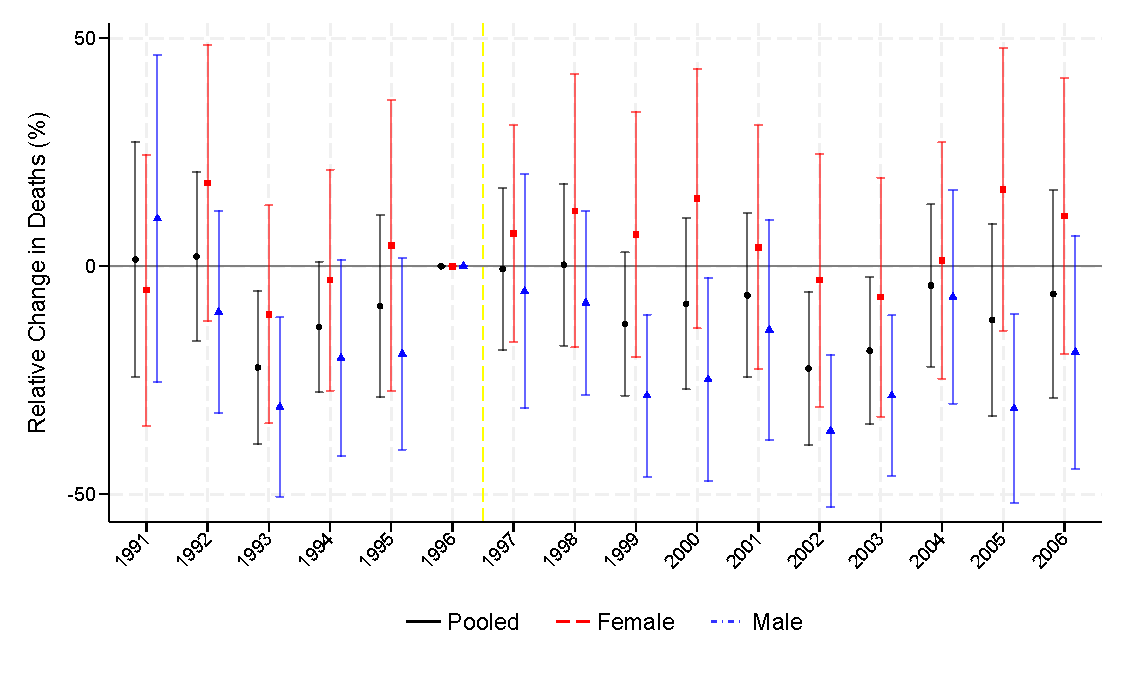
\includegraphics[width=0.49\textwidth]{figures/appendix/AF6d_ES_func_form_poisson.pdf}}

  \subfigure[AAMR]
{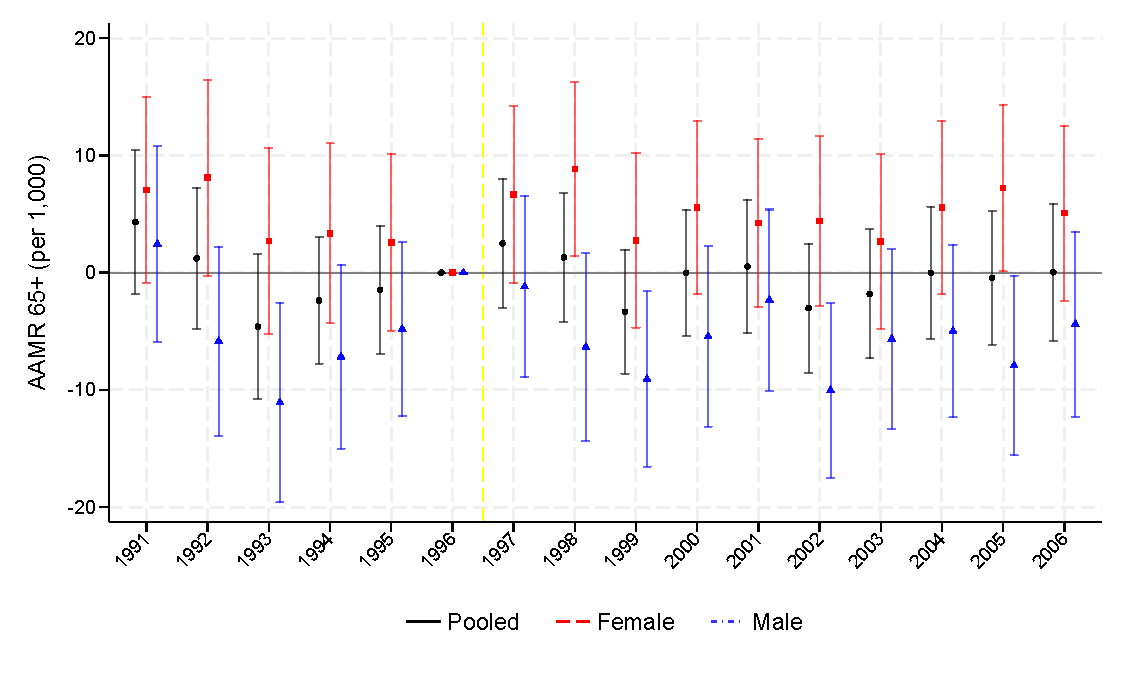
\includegraphics[width=0.49\textwidth]{figures/appendix/AF6e_aamr_col4.pdf}}

         \floatfoot{Notes: All panels display interaction coefficients between Progresa intensity in 1999, restricted to highly marginalized municipalities. 95\% confidence intervals shown. Panel~(a) shows the baseline specification. Panel~(b) shows the unweighted specification. Panel~(c) uses the natural log of the mortality rate (municipality-years with zero deaths are excluded); coefficients are multiplied by 100 and express the approximate percentage change in the mortality rate per unit increase in Progresa intensity. Panel~(d) uses Poisson with raw death counts as the outcome; coefficients are computed as $(\exp(\hat{\beta})-1)\times 100$ and express the percentage change in death counts per unit increase in intensity. Panel~(e) uses the Age-Adjusted Mortality Rate (AAMR) using each municipality's older adult population. All specifications include $\textit{Intensity}_{2005}$ and year indicators, municipality and year fixed effects, and Seguro Popular intensity controls.}
\end{figure}

\begin{figure}[H]
    \caption{Event Study: Stability of the Early-Phase (Intensity 1999) Coefficient to the Choice of Second-Phase Control}
    \label{af:beta0_stability}

{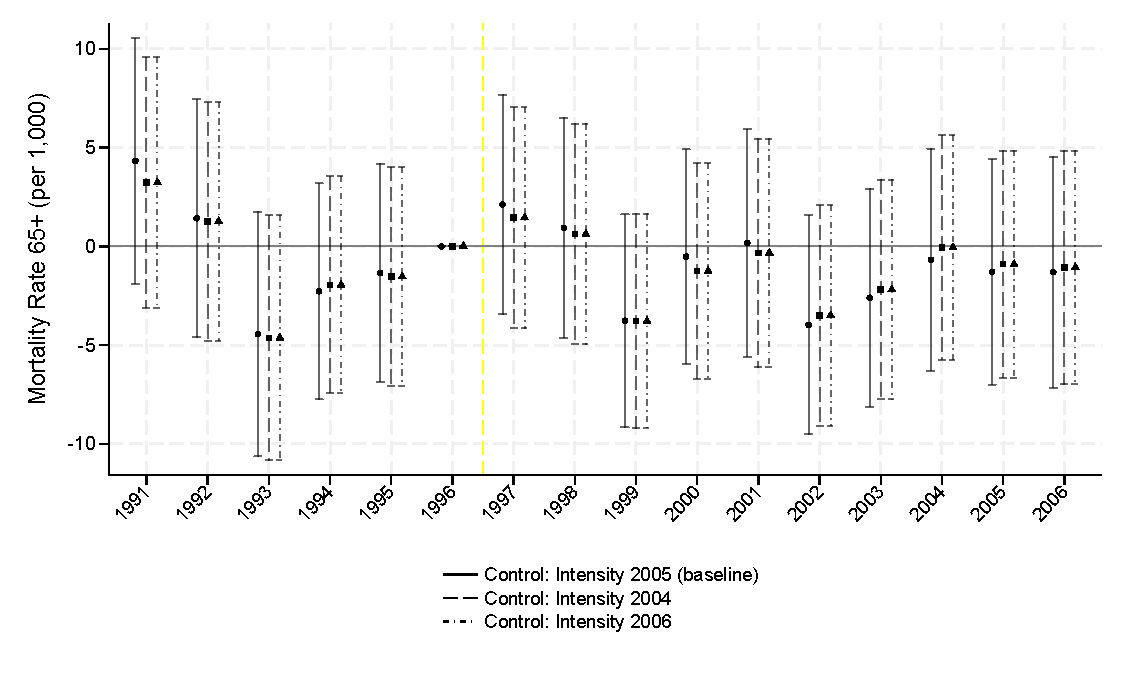
\includegraphics[width=0.85\textwidth]{figures/appendix/AF8_beta0_stability.pdf}}

         \floatfoot{Notes: This figure presents event-study estimates of the interaction between $\textit{Intensity}_{1999}$ and year indicators (reference year 1996) for the older-adult (65+) mortality rate per 1,000 inhabitants, under three specifications that each add a different later-phase (cumulative enrollment) control: the baseline specification controlling for $\textit{Intensity}_{2005}$, and specifications replacing it with the adjacent $\textit{Intensity}_{2004}$ and $\textit{Intensity}_{2006}$ snapshots. All specifications
         include Seguro Popular intensity, municipality and year fixed effects, and are weighted by the population aged 65 and older. The vertical line marks the program's 1997 roll-out. The sample is restricted to highly marginalized municipalities. 95\% confidence intervals shown.}
\end{figure}


\begin{figure}[H]
    \caption{Event Study: Effect of Progresa Enrollment Intensity on Mortality Rate by Sex and Sample, 1992--2002}
    \label{af:es_sample_compare}

%   \subfigure[Phase in 1998/1999 - All]
% {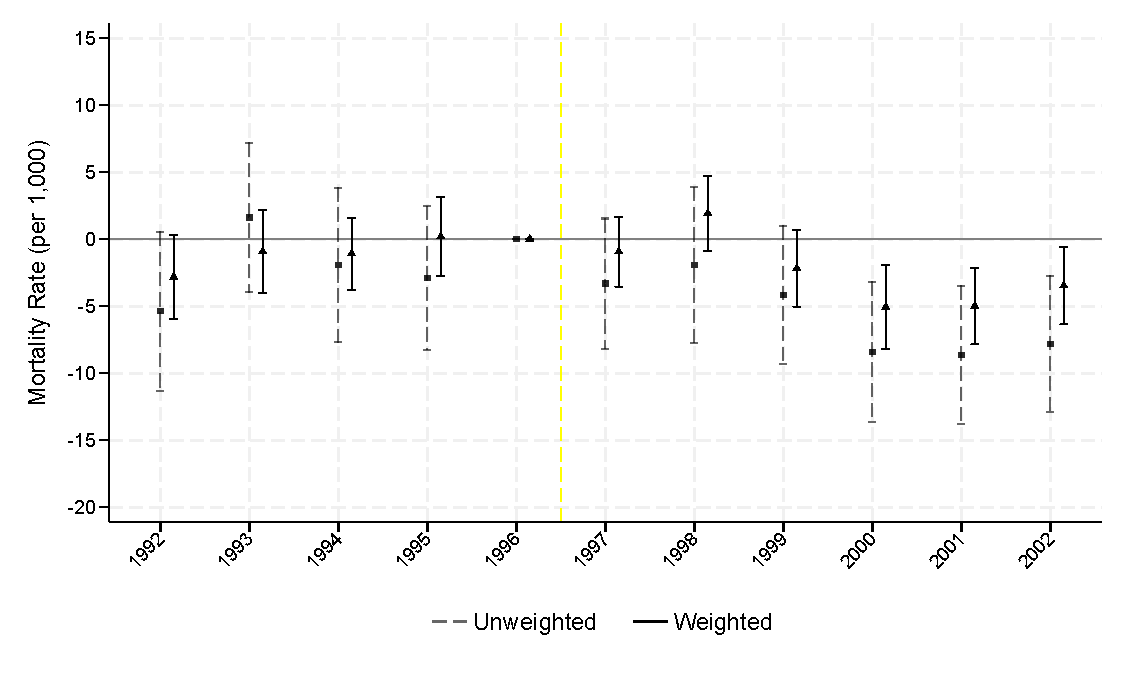
\includegraphics[width=0.49\textwidth]{figures/appendix/Figure_6_emr65_BR.pdf}}
%     \subfigure[Highly Marginalized - All]
% {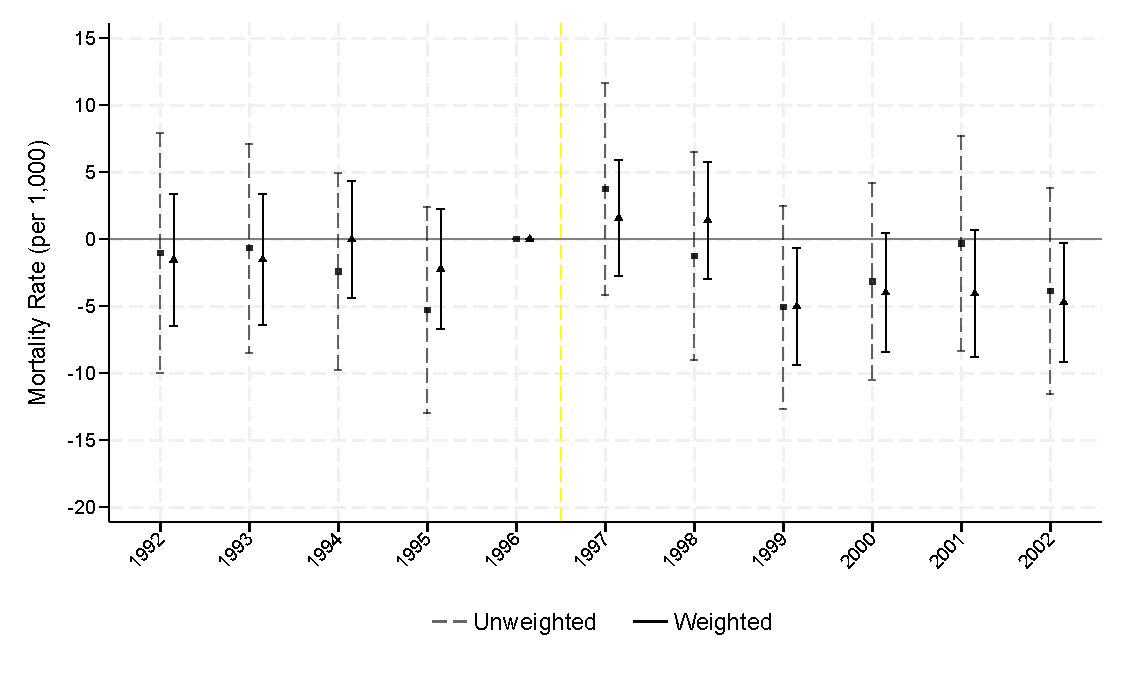
\includegraphics[width=0.49\textwidth]{figures/appendix/Figure_6_emr65_HighMarg.pdf}}


\subfigure[Phase in 1998/1999 - Females]
{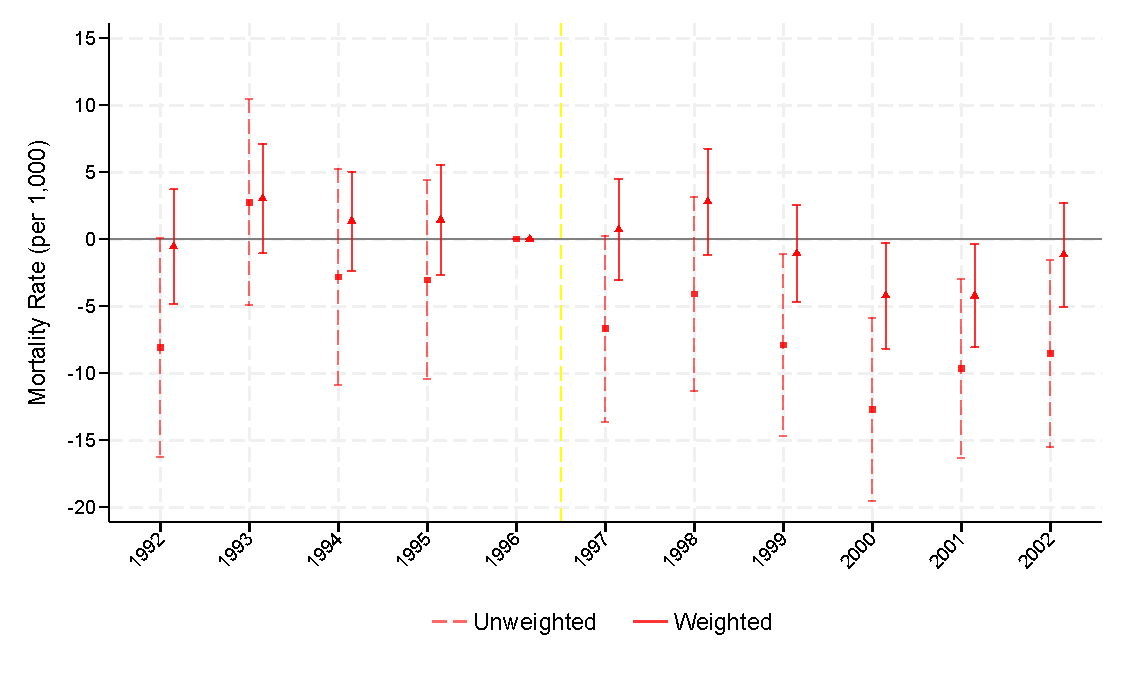
\includegraphics[width=0.49\textwidth]{figures/appendix/AF9a_emr65f_BR.pdf}}
\subfigure[Highly Marginalized - Females]
     {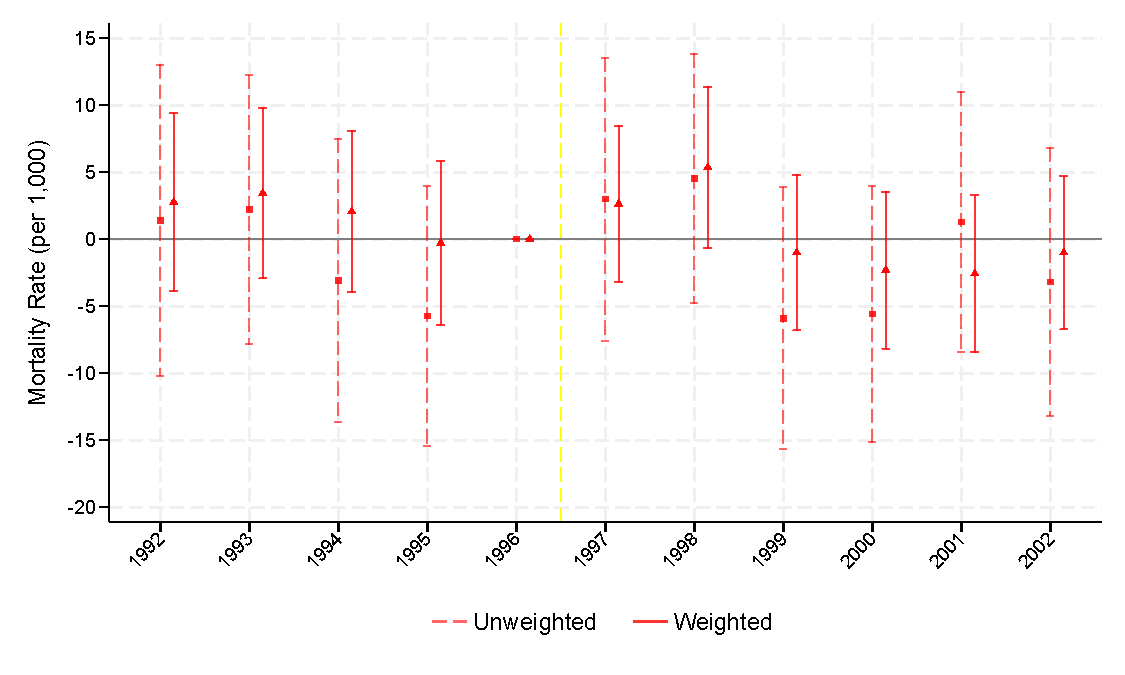
\includegraphics[width=0.49\textwidth]{figures/appendix/AF9b_emr65f_HighMarg.pdf}}

\subfigure[Phase in 1998/1999 - Males]
{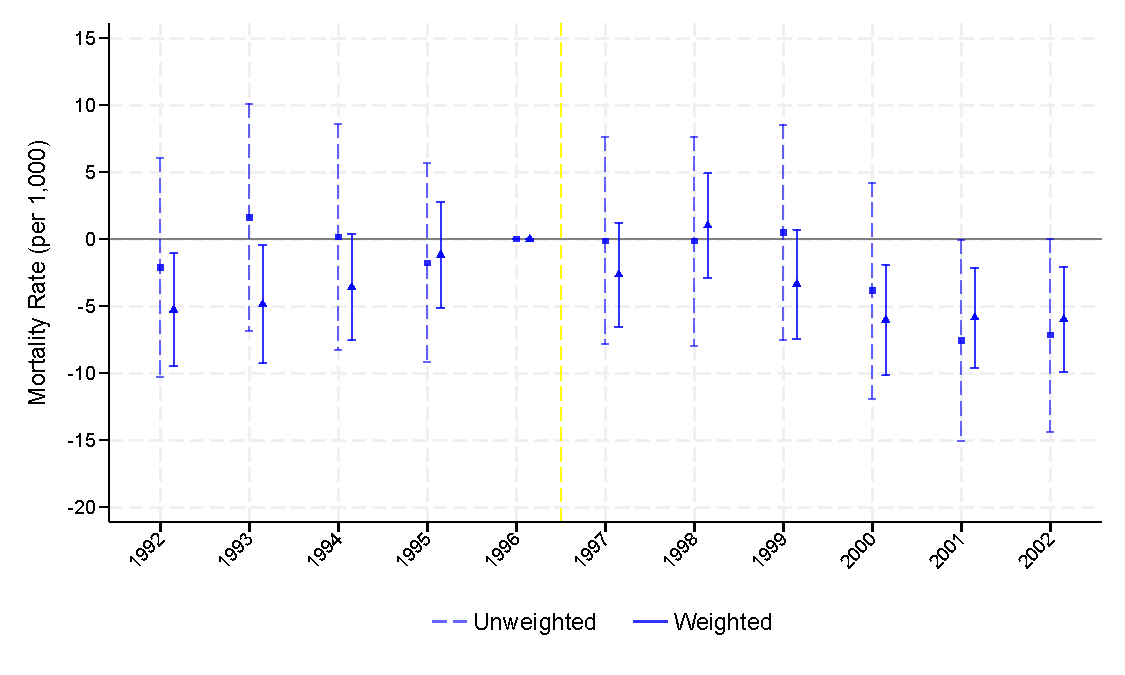
\includegraphics[width=0.49\textwidth]{figures/appendix/AF9c_emr65m_BR.pdf}}
 \subfigure[Highly Marginalized - Males]
{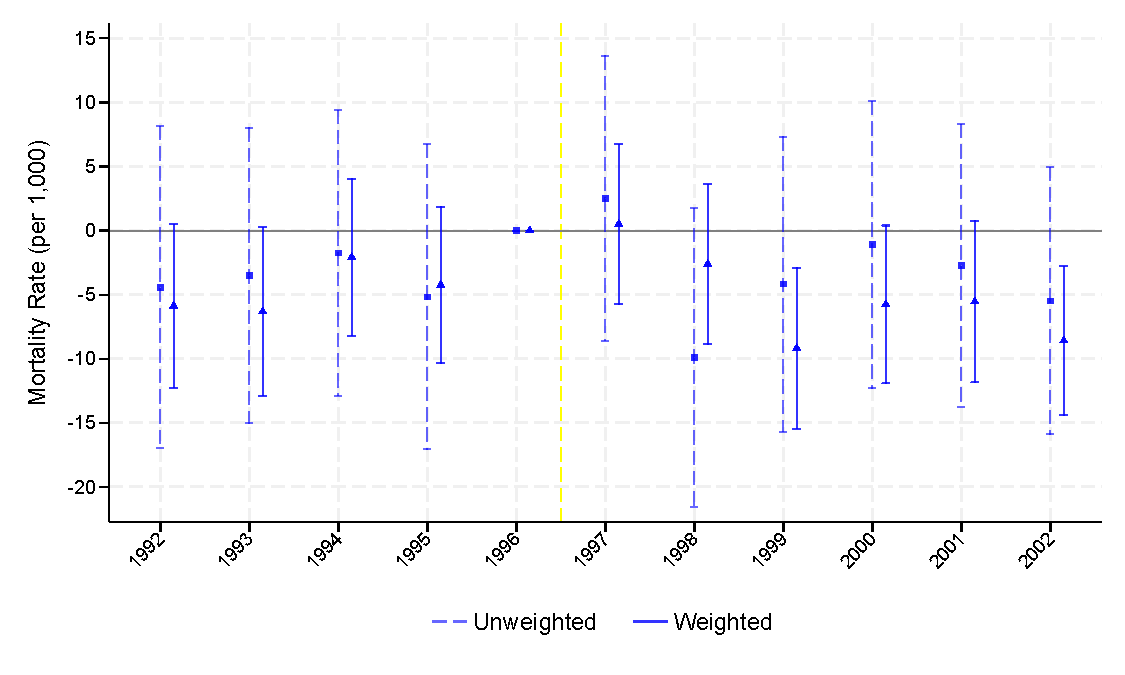
\includegraphics[width=0.49\textwidth]{figures/appendix/AF9d_emr65m_HighMarg.pdf}}

         \floatfoot{Notes: This figure compares event study estimates across the two sample definitions used in this paper and in Barham and Rowberry (2013). Left panels (BR) restrict to municipalities incorporated into Progresa in 1998 or 1999; right panels (HM) restrict to highly marginalized municipalities. All regressions include municipality and year fixed effects; the reference year is 1996; the period is 1992--2002. 95\% confidence intervals shown.}
\end{figure}



% \begin{figure}[H]
%     \caption{Event Study: Effect of Progresa Enrollment Intensity on the 65+ Population}
%     \label{af:migration_es}

% \subfigure[Levels]
% {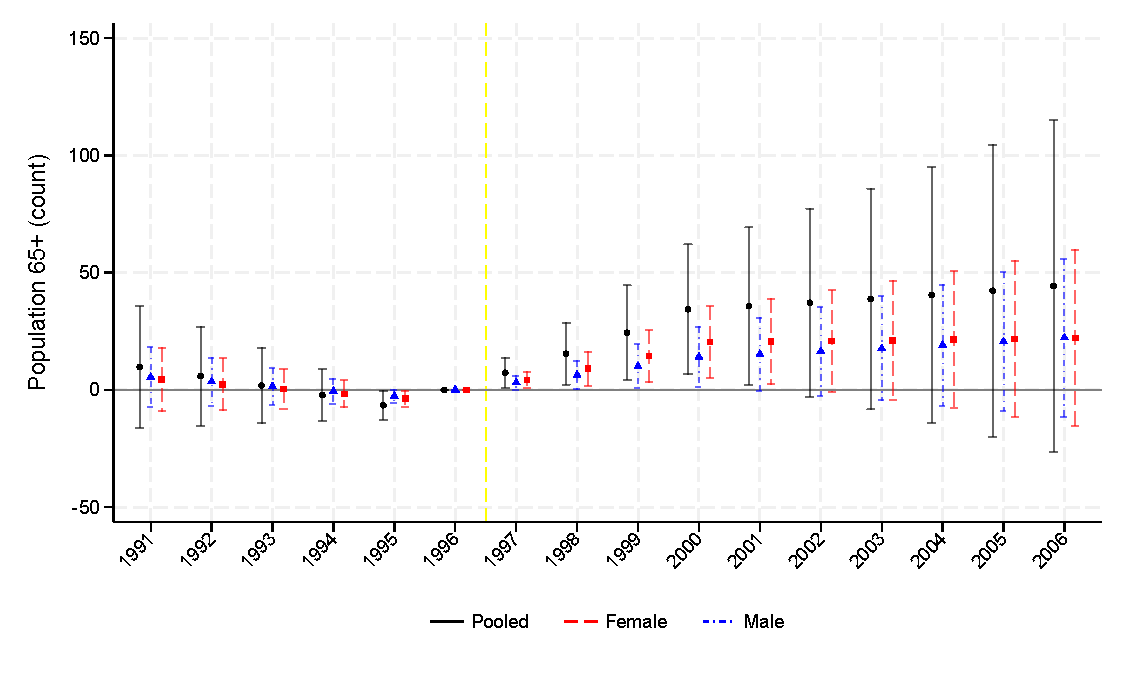
\includegraphics[width=0.49\textwidth]{figures/appendix/AF_migration_es.pdf}}
% \subfigure[Log]
% {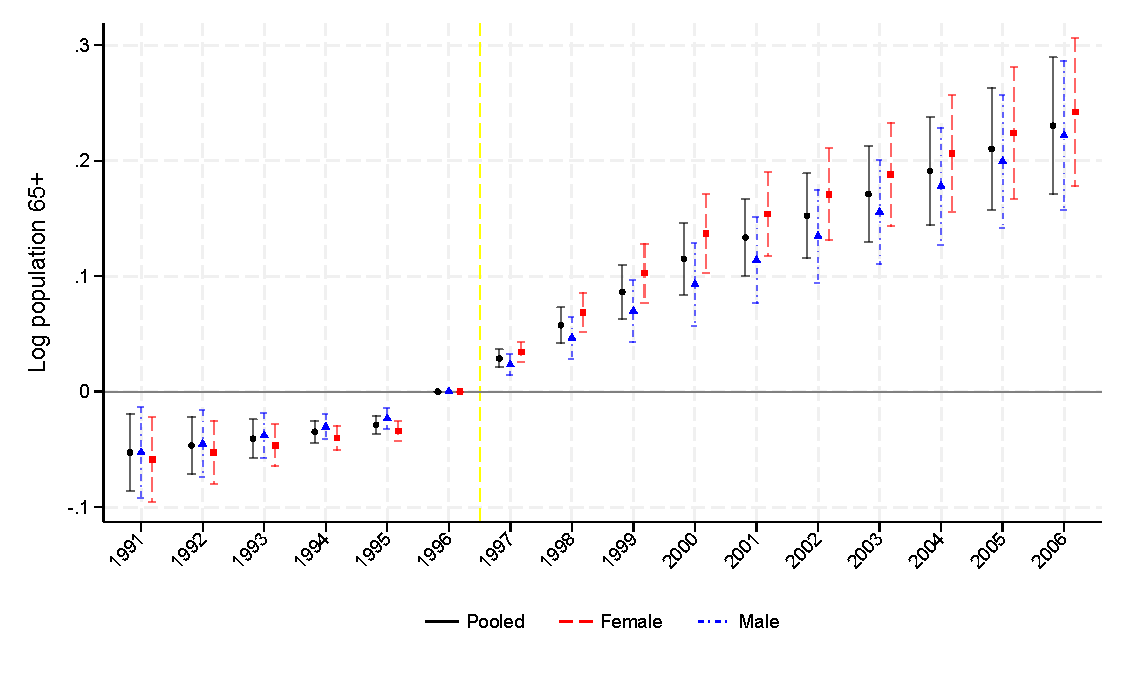
\includegraphics[width=0.49\textwidth]{figures/appendix/AF_migration_es_log.pdf}}
% \subfigure[Poisson]
% {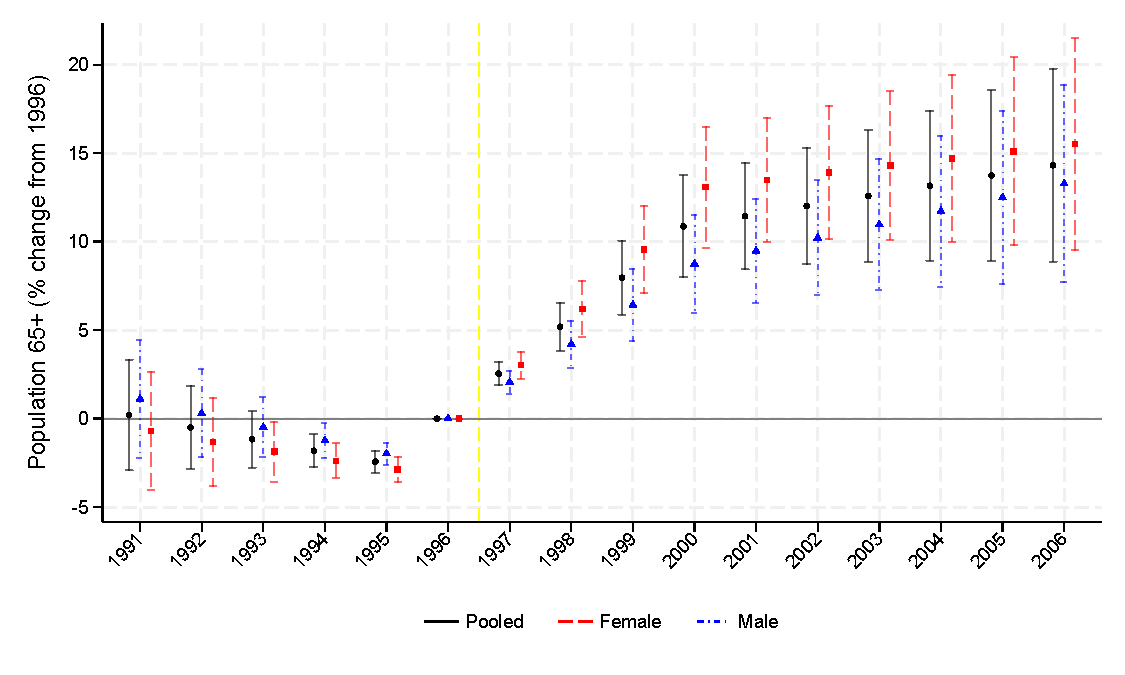
\includegraphics[width=0.49\textwidth]{figures/appendix/AF_migration_es_poisson.pdf}}

%          \floatfoot{Notes: This figure presents event-study estimates of the interaction between $\textit{Intensity}_{1999}$ and year indicators (reference year 1996) for the 65+ population, pooled, female, and male, as a check on whether any apparent migration effect (Appendix Tables~\ref{at:migration_rob}--\ref{at:migration_rob_agefe}) is a pre-existing trend rather than a post-1997 program effect. Panel~(a) uses the population count; panel~(b) uses log population; panel~(c) uses Poisson pseudo-maximum likelihood, with coefficients computed as $(\exp(\hat\beta_t)-1)\times 100$, the percentage change in population at each year relative to 1996. Same specification as the mortality event studies: municipality and year fixed effects, Seguro Popular intensity, clustered at the municipality level. The sample is restricted to highly marginalized municipalities. 95\% confidence intervals shown.}
% \end{figure}

% ============================================================
% >>> TEMPORARY -- FOR REVIEW ONLY, remove after checking. <<<
% Robustness check requested by the coauthor: Figure 2 re-estimated
% with the sample restricted to 1991--2005 (drops 2006, the year a
% pension component for ages 70+ was added to Progresa), to check
% whether that one year is doing any work in the main event study.
% Built in codes/04_extra_robustness.do (right before log close) --
% run that block first to generate the three
% figures/appendix/Figure_2_{pooled,female,male}_through2005.pdf files
% before compiling this file.
% ============================================================

% \begin{figure}[H]
%     \caption{Event Study: Effect of Progresa Enrollment Intensity on Mortality Rate by Sex, Restricted to 1991--2005}
%     \label{af:f2_through2005}
%     \subfigure[Pooled]
%      {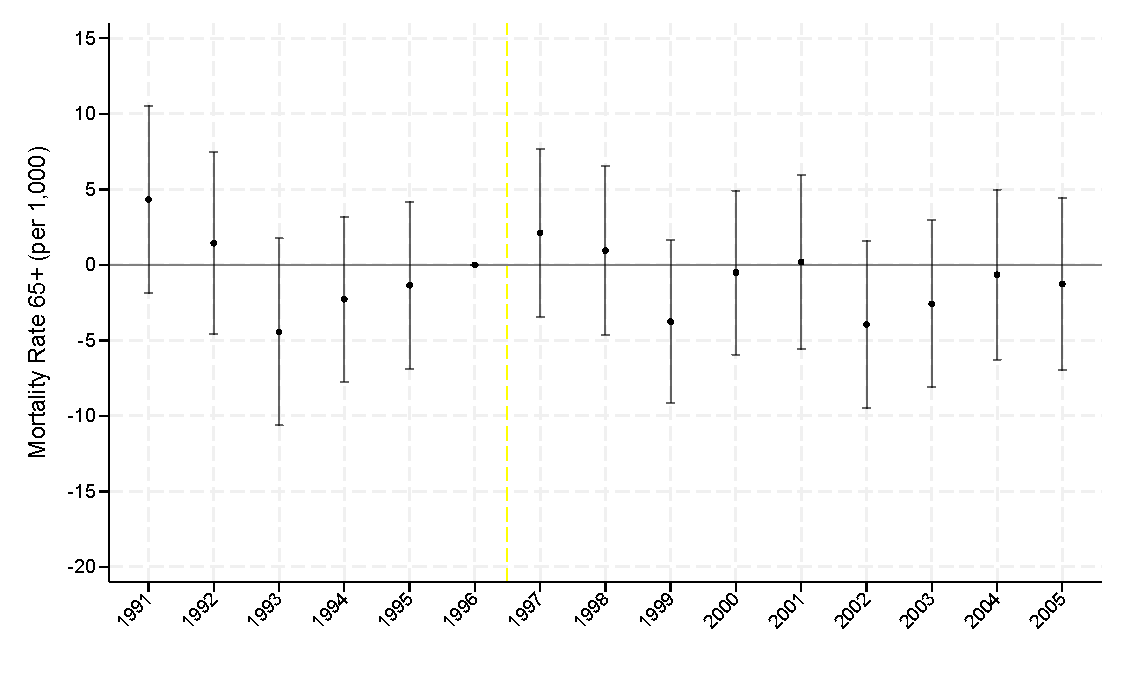
\includegraphics[width=0.6\textwidth]{figures/appendix/Figure_2_pooled_through2005.pdf}}
%
%     \subfigure[Female]
% {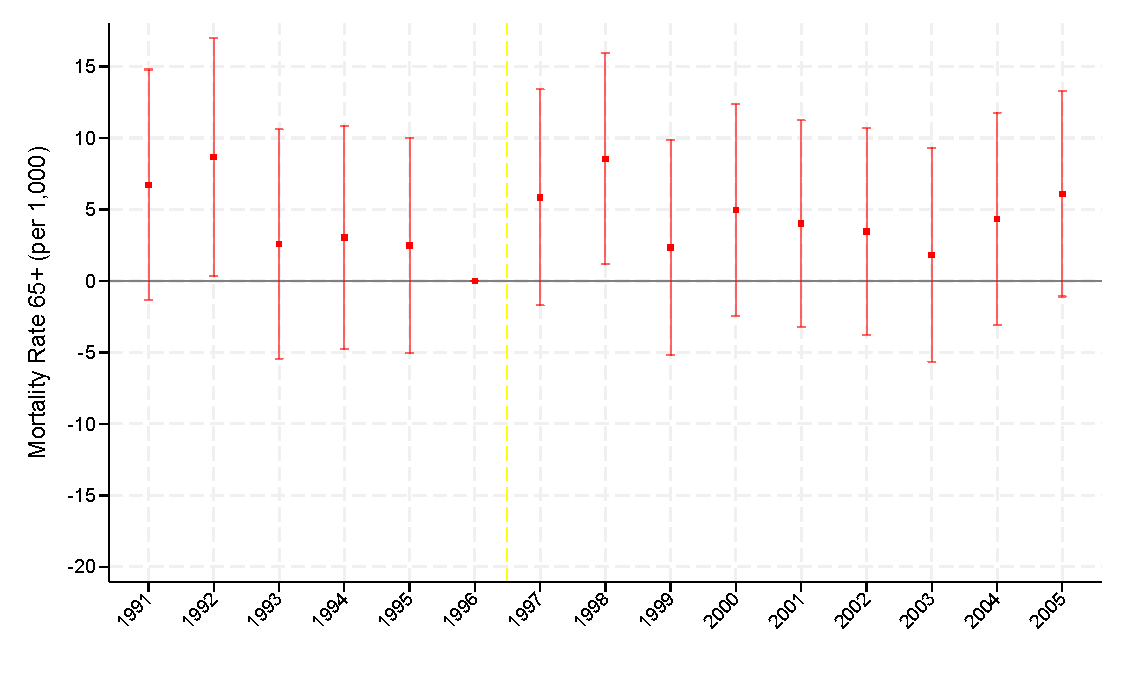
\includegraphics[width=0.49\textwidth]{figures/appendix/Figure_2_female_through2005.pdf}}
%     \subfigure[Male]
%      {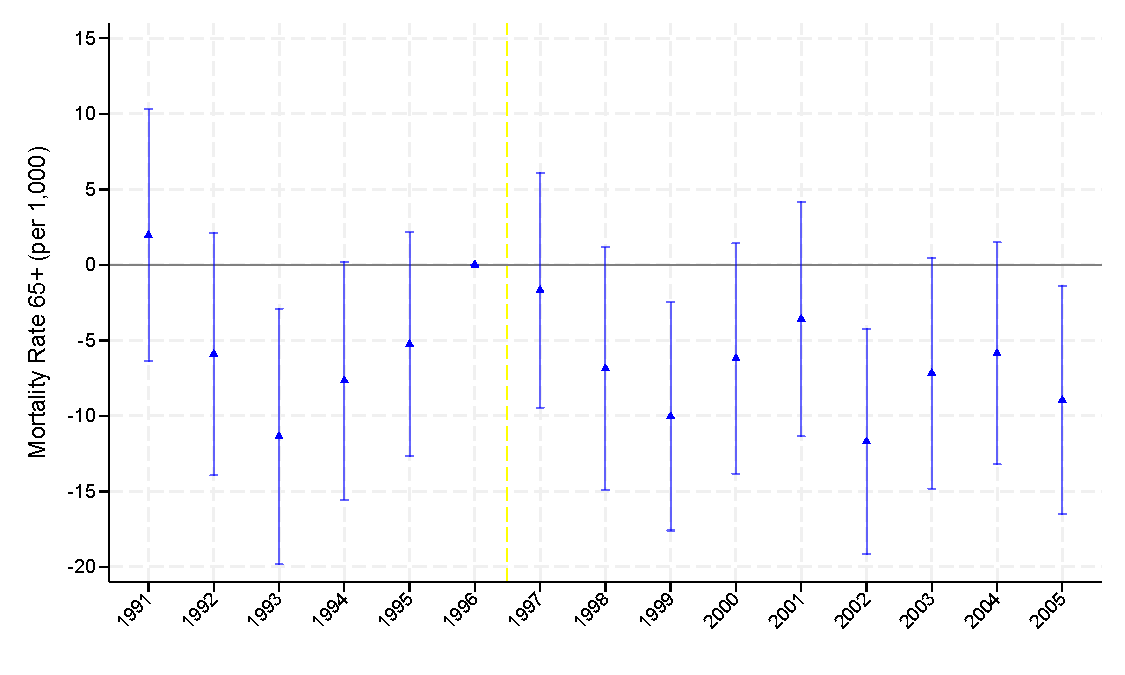
\includegraphics[width=0.49\textwidth]{figures/appendix/Figure_2_male_through2005.pdf}}
%          \floatfoot{Notes: This figure reproduces Figure~\ref{f:es_dd_sex_no_weight} (the main event study) with the sample restricted to 1991--2005, dropping 2006 -- the year a pension component for ages 70 and older was added to \textit{Progresa} -- as a robustness check on the panel's endpoint. Panels~(a)--(c) display the interaction coefficients between Progresa intensity in 1999 and year indicators for the pooled, female, and male samples, respectively. All specifications include the $\textit{Intensity}_{2005}$ interaction, municipality and year fixed effects, and Seguro Popular intensity. Standard errors are clustered at the municipality level. The reference year is 1996. The sample is restricted to highly marginalized municipalities. Regressions are weighted by the population aged 65 and older. 95\% confidence intervals shown.}
% \end{figure}
% >>> END TEMPORARY BLOCK <<<

% ============================================================
% Dose-response "cloud" and Barham--Rowberry decomposition, suggested by
% Andrew Goodman-Bacon (October 2026), following Callaway, Goodman-Bacon
% and Sant'Anna (2025). Built in codes/04_extra_robustness.do (the block
% right before the cause-of-death section): run it first to generate the
% AF_cloud_*, AF_twfe_weights_* and AF_br_leftover_* files.
% ============================================================

\begin{figure}[H]
    \caption{Change in Older Adults' Mortality by Early-Phase Enrollment Intensity}
    \label{af:cloud_mortality}

    \subfigure[Change after 1997]
     {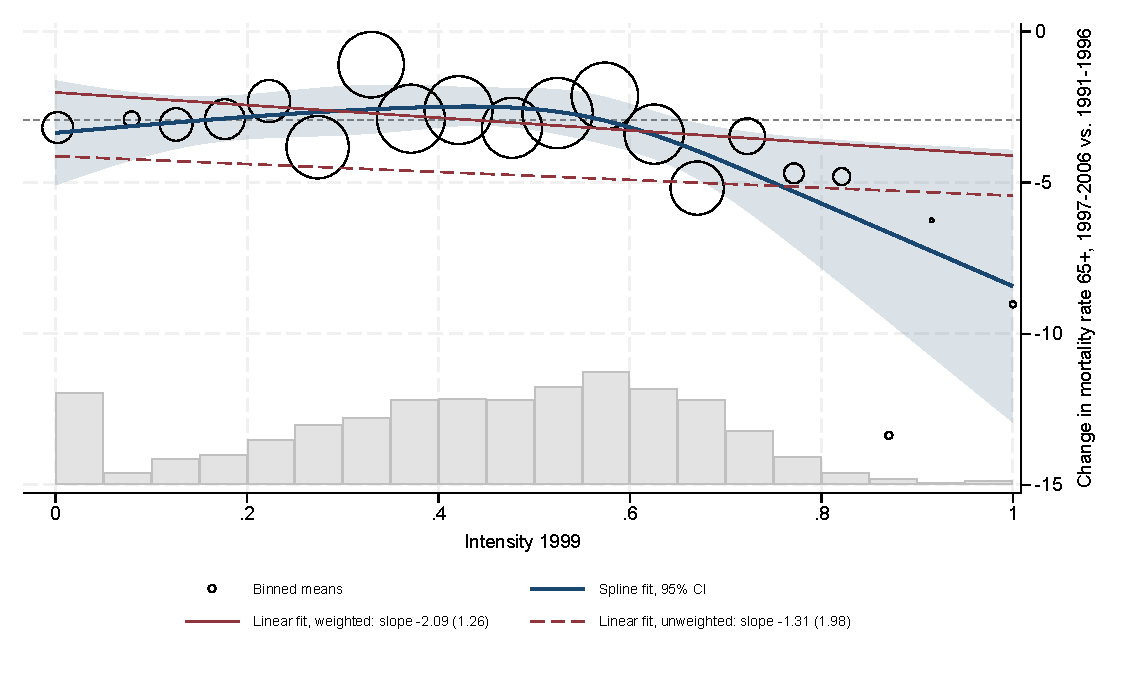
\includegraphics[width=0.49\textwidth]{figures/appendix/AF_cloud_post_plain.pdf}}
    \subfigure[Change after 1997, net of later-phase enrollment]
     {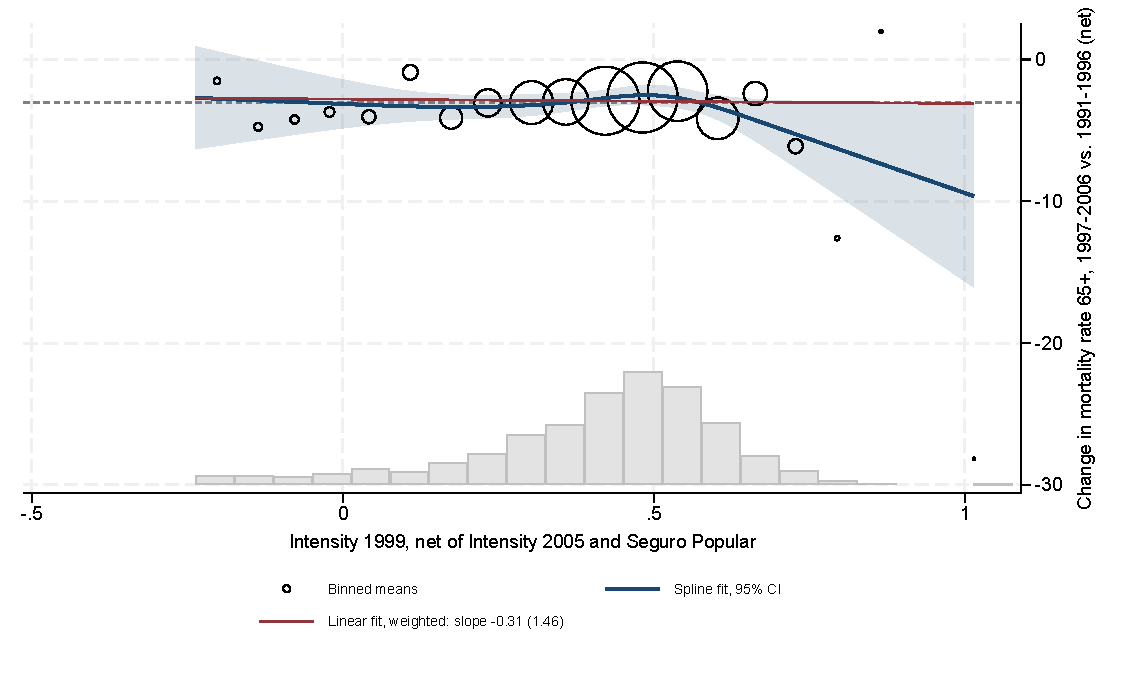
\includegraphics[width=0.49\textwidth]{figures/appendix/AF_cloud_post_cond.pdf}}
    \subfigure[Pre-period placebo]
     {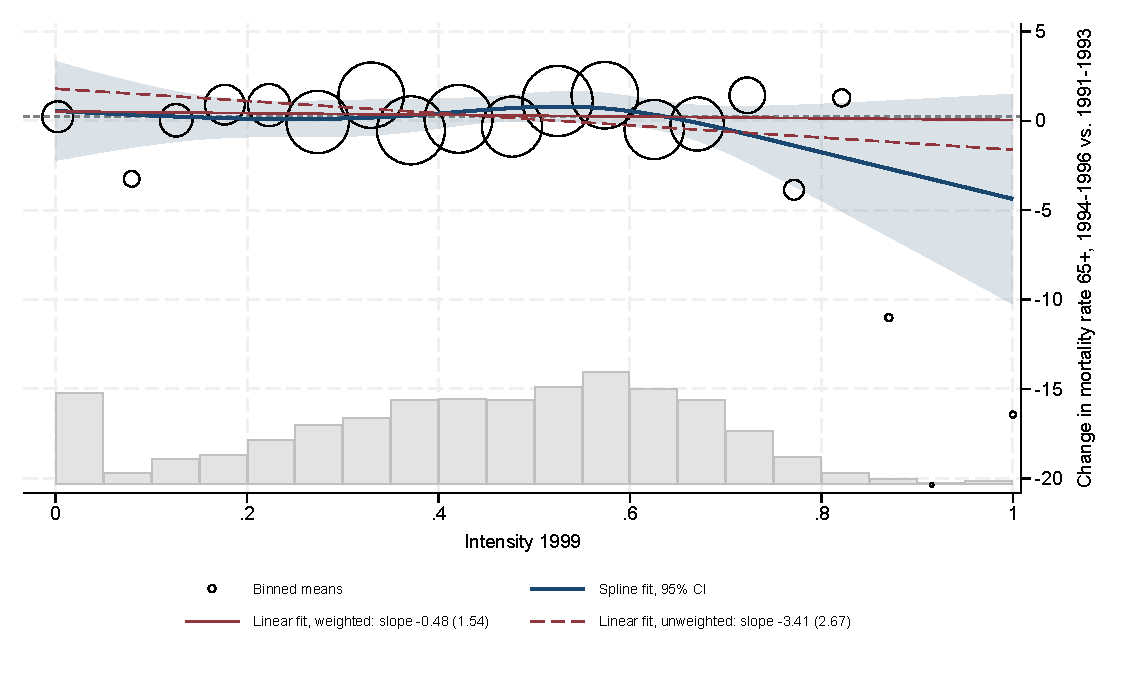
\includegraphics[width=0.49\textwidth]{figures/appendix/AF_cloud_pre_plain.pdf}}
    \subfigure[Pre-period placebo, net of later-phase enrollment]
     {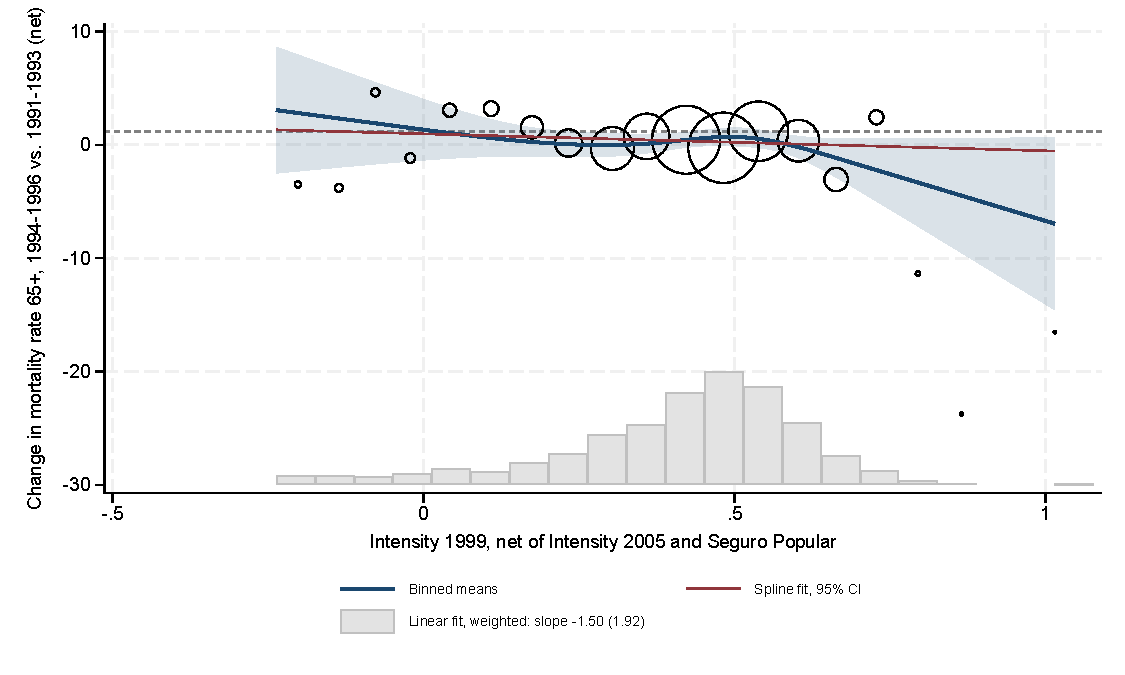
\includegraphics[width=0.49\textwidth]{figures/appendix/AF_cloud_pre_cond.pdf}}

         \floatfoot{Notes: Following \citet{callaway2025continuous}, each panel plots the change in each highly marginalized municipality's mortality rate for adults aged 65 and older (deaths per 1,000) against its \textit{Progresa} enrollment intensity in 1999. In panels~(a) and (b), the change is the 1997--2006 mean minus the 1991--1996 mean; panels~(c) and (d) are a placebo using the change from 1991--1993 to 1994--1996, before the program began. Circles are means within 20 equal-width intensity bins, weighted by the 1991--1996 average population aged 65 and older, with area proportional to bin population. The navy curve is a restricted cubic spline (four knots) with its 95\% confidence interval; the solid and dashed maroon lines are the population-weighted and unweighted linear fits, with slopes and robust standard errors in the legend. The dashed grey line marks the mean change in the lowest-intensity decile: because every municipality was eventually treated, changes are identified only relative to the least-treated municipalities, and differences across intensity levels are causal effects only under strong parallel trends. Grey bars show the distribution of municipalities by intensity. In panels~(b) and (d), both axes are net of $\textit{Intensity}_{2005}$ and post-1997 Seguro Popular intensity (population-weighted), with means added back; the weighted slope in panel~(b) is the two-period analog of $\beta_0$ in Table~\ref{t:did_age}, column~(1), and the weighted slope in panel~(a) that of the specification without later-phase controls in Appendix Table~\ref{at:no_control_sex}.}
\end{figure}

\begin{figure}[H]
    \caption{Implicit Regression Weights and the Distribution of Early-Phase Enrollment Intensity}
    \label{af:twfe_weights}

    \subfigure[Intensity in 1999]
     {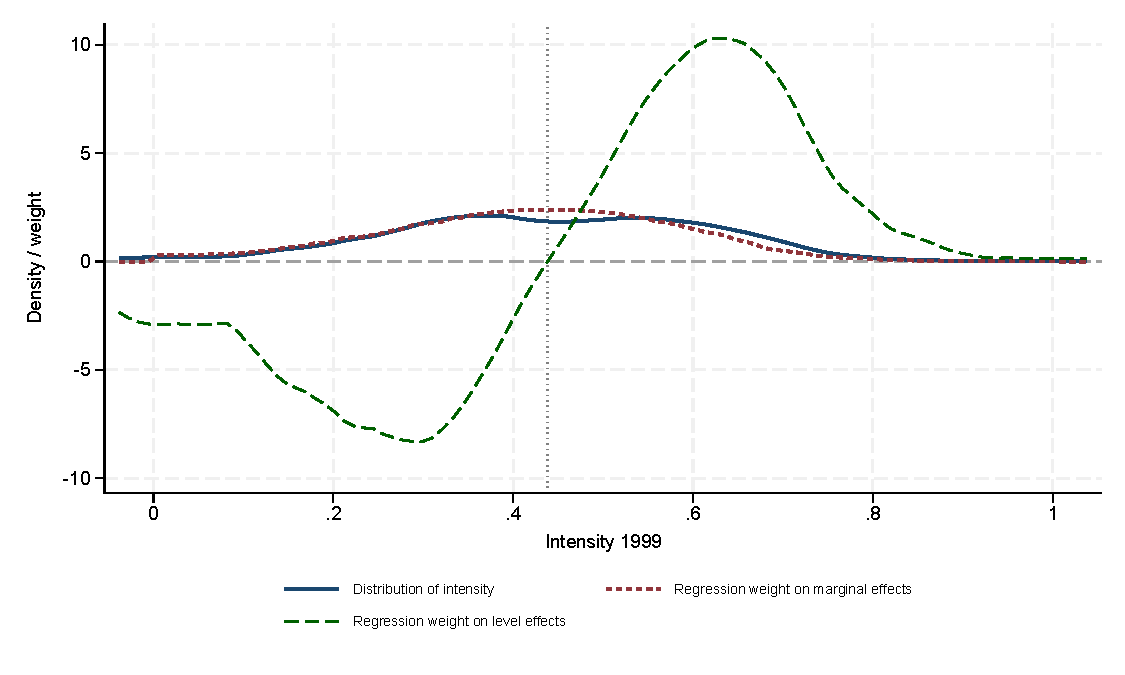
\includegraphics[width=0.49\textwidth]{figures/appendix/AF_twfe_weights_plain.pdf}}
    \subfigure[Intensity in 1999, net of later-phase enrollment]
     {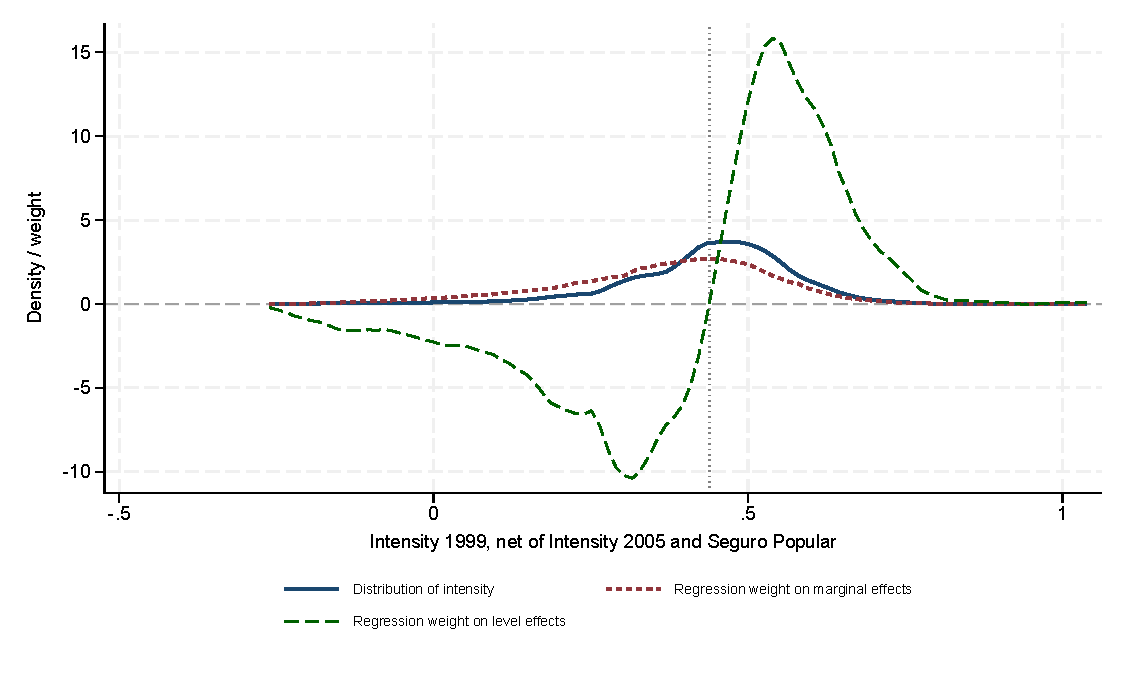
\includegraphics[width=0.49\textwidth]{figures/appendix/AF_twfe_weights_cond.pdf}}

         \floatfoot{Notes: This figure shows how a linear difference-in-differences regression on $\textit{Intensity}_{1999}$ weights effects at different intensity levels \citep[Table~1]{callaway2025continuous}. The solid line is the distribution (kernel density) of intensity across highly marginalized municipalities. The dotted line is the weight the regression places on the marginal effect of intensity at each level, $w(l)=E[(D-E[D])\,\mathbf{1}\{D\geq l\}]/\mathrm{Var}(D)$; the dashed line is the weight it places on the level effect at each intensity, $(l-E[D])\,f(l)/\mathrm{Var}(D)$, which is negative below the mean (vertical line). With no untreated municipalities, the marginal-effect weights are non-negative, integrate to one, and coincide with the density when intensity is normally distributed. Panel~(b) uses intensity net of $\textit{Intensity}_{2005}$ and Seguro Popular intensity, the variation used by the specification with later-phase controls. All quantities are weighted by the 1991--1996 average population aged 65 and older.}
\end{figure}

\begin{figure}[H]
    \caption{Change in Older Adults' Mortality by Barham and Rowberry's Treatment}
    \label{af:cloud_br}

    \subfigure[Unweighted]
     {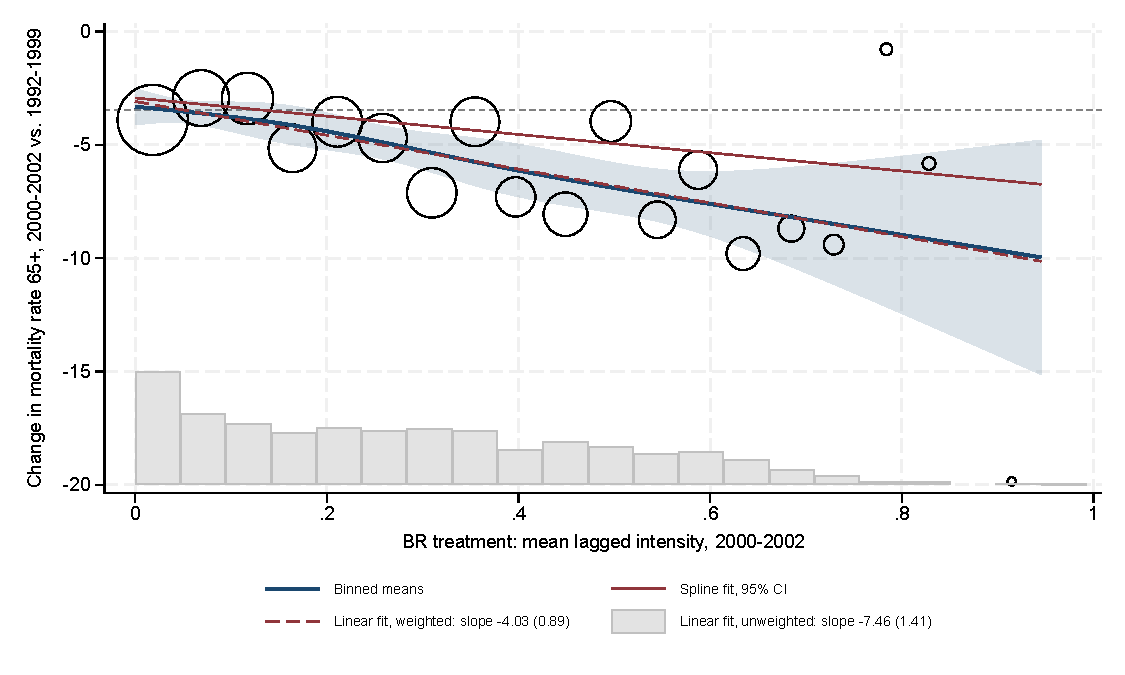
\includegraphics[width=0.49\textwidth]{figures/appendix/AF_cloud_br_uw.pdf}}
    \subfigure[Weighted by population aged 65 and older]
     {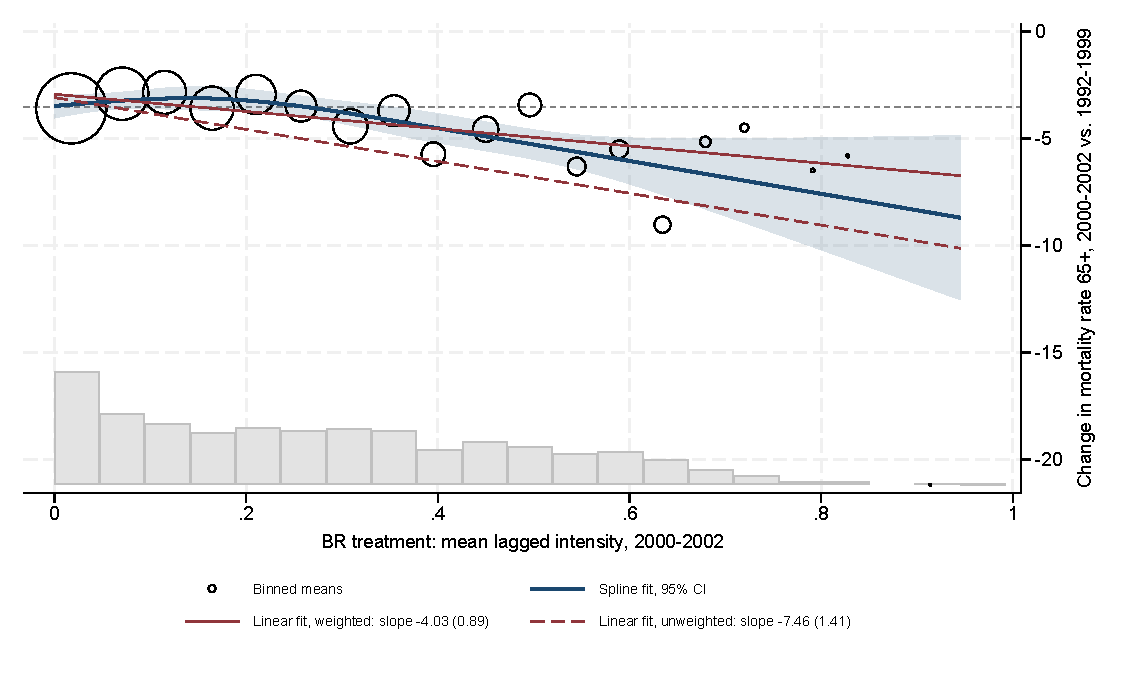
\includegraphics[width=0.49\textwidth]{figures/appendix/AF_cloud_br_w.pdf}}

         \floatfoot{Notes: This figure shows the raw data behind the design of \citet{BarhamRowberry2013JDE}, in the format of Appendix Figure~\ref{af:cloud_mortality}: municipalities first incorporated into \textit{Progresa} in 1998 or 1999, observed over 1992--2002, with treatment equal to enrollment intensity lagged two years. The vertical axis is each municipality's change in the mortality rate for adults aged 65 and older (deaths per 1,000), from its 1992--1999 mean, when the lagged treatment is zero, to its 2000--2002 mean. The horizontal axis is the municipality's mean lagged treatment over 2000--2002, that is, its mean enrollment intensity in 1998--2000, which is close to $\textit{Intensity}_{1999}$. Nothing is adjusted: unlike Appendix Figure~\ref{af:br_leftover}, there are no fixed effects or controls, and negative values on the horizontal axis do not occur. Circles are means within 20 equal-width bins of the horizontal axis. Panel~(a) weights municipalities equally, as \citet{BarhamRowberry2013JDE} do, and circle area is proportional to the number of municipalities in the bin; panel~(b) weights by the 1992--1999 average population aged 65 and older, and circle area is proportional to bin population. Both panels report the same two linear fits, whichever weighting the circles use: the solid maroon line is the population-weighted fit and the dashed maroon line the unweighted fit, with slopes and robust standard errors in the legend. The navy curve is a restricted cubic spline (four knots) with its 95\% confidence interval, estimated with the weights of the panel. The dashed grey line marks the mean change in the lowest-intensity decile, the benchmark against which changes at higher intensities are read. Grey bars show the distribution of municipalities by intensity, identical in both panels; the high-intensity tail is sparse, so its circles and the right end of the curve are imprecise. This two-period comparison only approximates their regression; Appendix Table~\ref{at:br_leftover} and Appendix Figure~\ref{af:br_leftover} report the exact estimates.}
\end{figure}

\begin{figure}[H]
    \caption{Barham and Rowberry's Identifying Variation Before and After Removing Early-Phase Intensity}
    \label{af:br_leftover}

    \subfigure[Unweighted, fixed effects only]
     {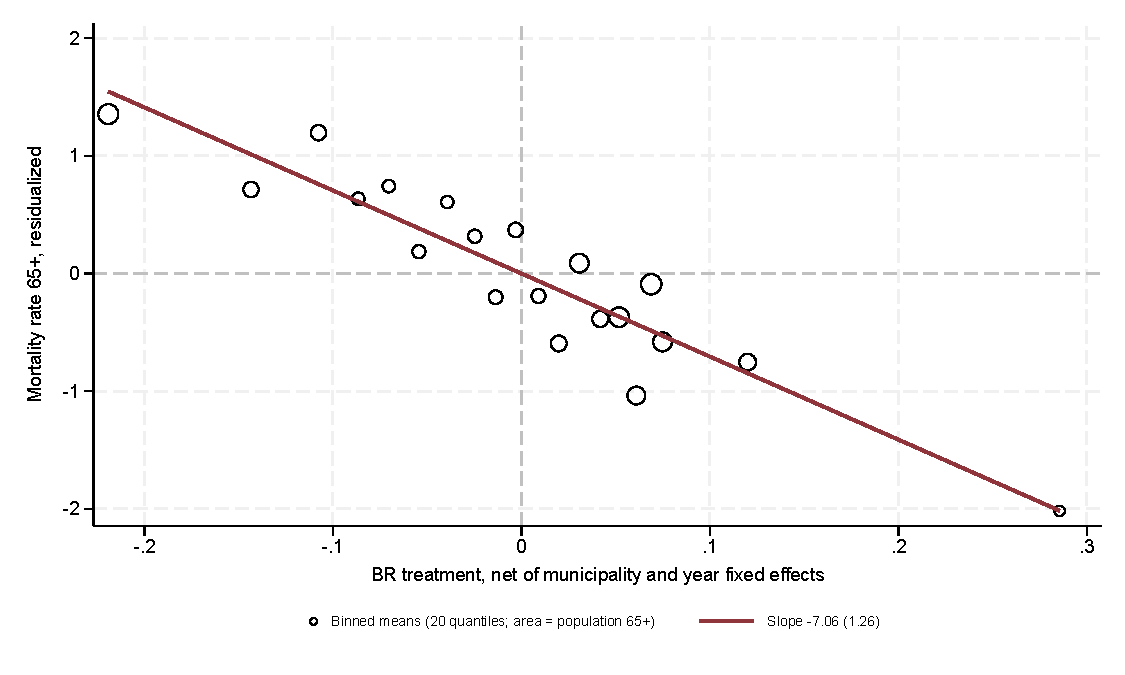
\includegraphics[width=0.49\textwidth]{figures/appendix/AF_br_leftover_fe_uw.pdf}}
    \subfigure[Unweighted, net of Intensity 1999 $\times$ year]
     {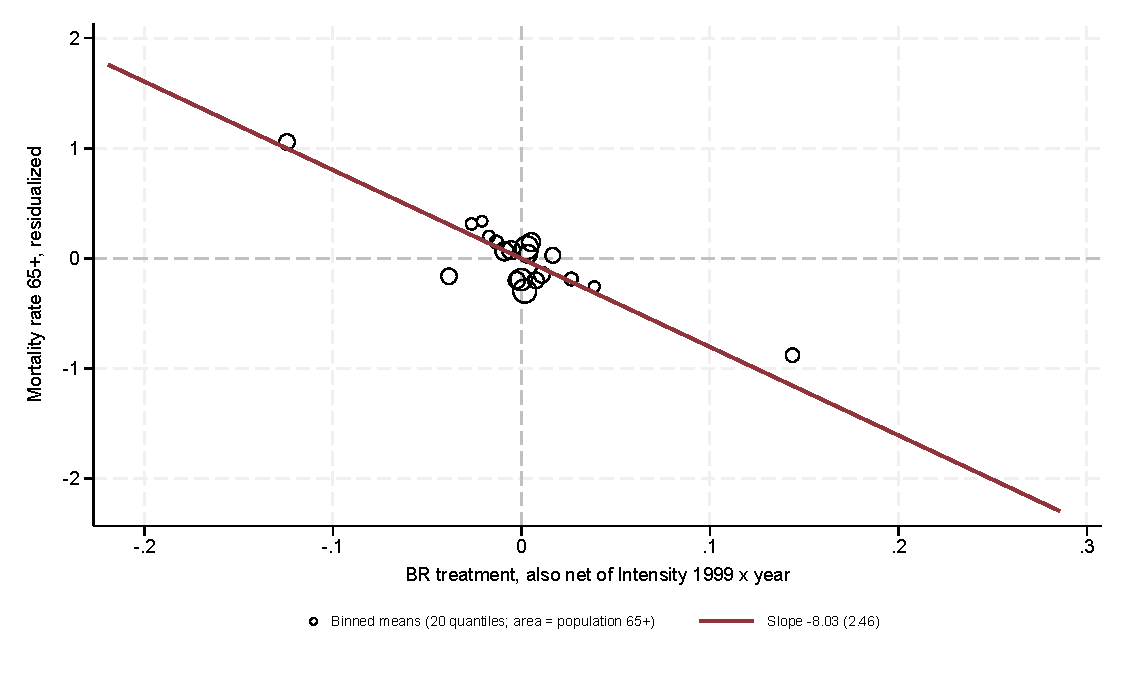
\includegraphics[width=0.49\textwidth]{figures/appendix/AF_br_leftover_i99_uw.pdf}}
    \subfigure[Weighted, fixed effects only]
     {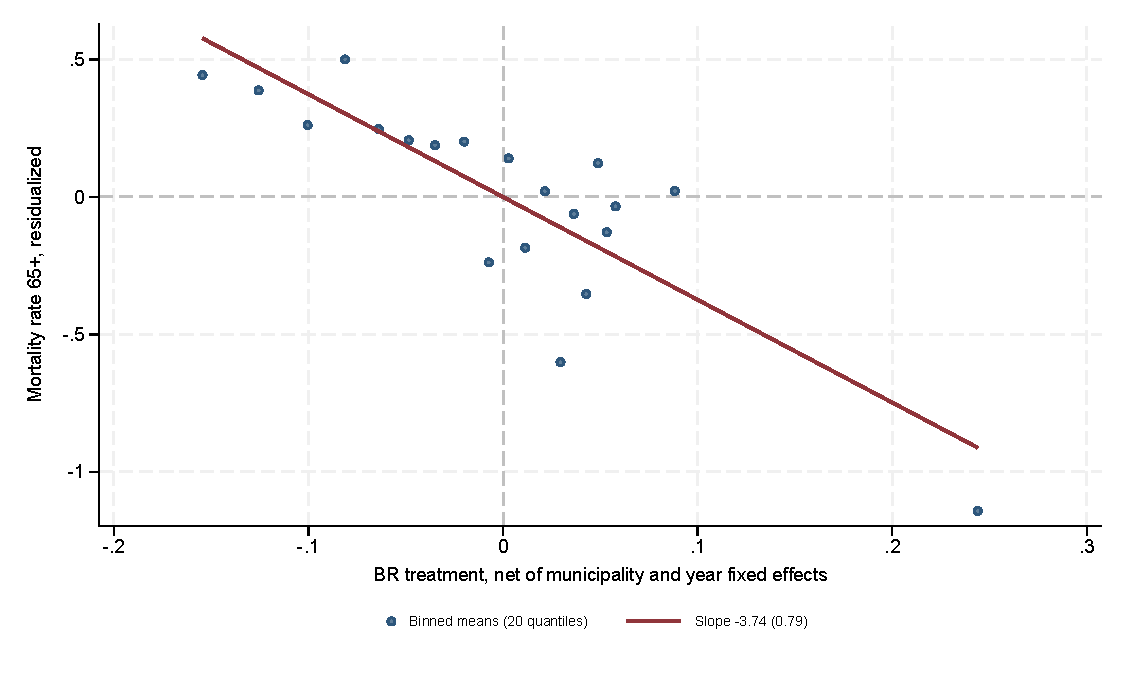
\includegraphics[width=0.49\textwidth]{figures/appendix/AF_br_leftover_fe_w.pdf}}
    \subfigure[Weighted, net of Intensity 1999 $\times$ year]
     {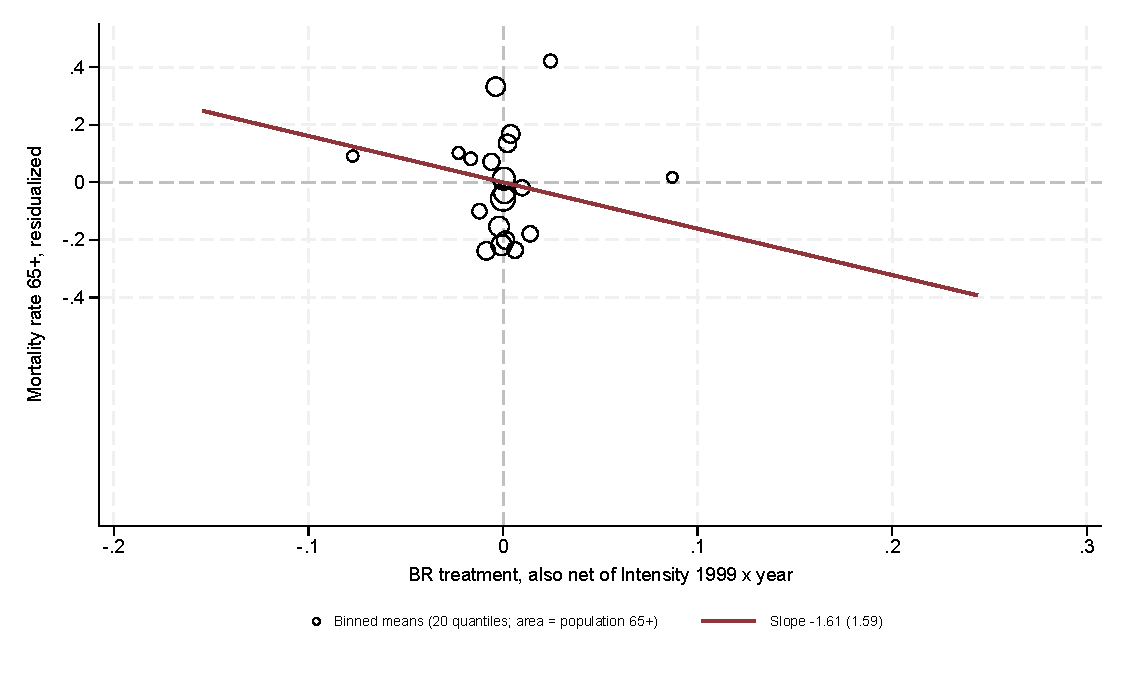
\includegraphics[width=0.49\textwidth]{figures/appendix/AF_br_leftover_i99_w.pdf}}

         \floatfoot{Notes: Each panel is a binned scatter (20 quantile bins; circle area proportional to the bin's average population aged 65 and older) of the mortality rate for adults aged 65 and older (deaths per 1,000) against the treatment of \citet{BarhamRowberry2013JDE}, enrollment intensity lagged two years, in their sample (municipalities first incorporated in 1998 or 1999) and period (1992--2002). In panels~(a) and (c), both variables are net of municipality and year fixed effects, so the slope is their two-way fixed effects estimate. In panels~(b) and (d), both are also net of $\textit{Intensity}_{1999}$ interacted with year indicators, the variation our event study uses, so by the Frisch--Waugh--Lovell theorem the slope is their estimate computed only from the part of their treatment that our design does not use. Panels~(a) and (b) are unweighted, as in their paper; panels~(c) and (d) are weighted by population aged 65 and older. Axes are identical within each row, so the narrower horizontal spread in the right-hand panel shows how much of their treatment variation our design shares. Slopes and standard errors clustered at the municipality level are reported in the legend and match Appendix Table~\ref{at:br_leftover}, Panel~A. Appendix Figures~\ref{af:br_trim} and~\ref{af:br_size} probe whether these slopes are driven by the tails of the residualized treatment or by small municipalities.}
\end{figure}

\begin{figure}[H]
    \caption{Barham and Rowberry's Estimate After Trimming the Tails of the Identifying Variation}
    \label{af:br_trim}

    \subfigure[Unweighted]
     {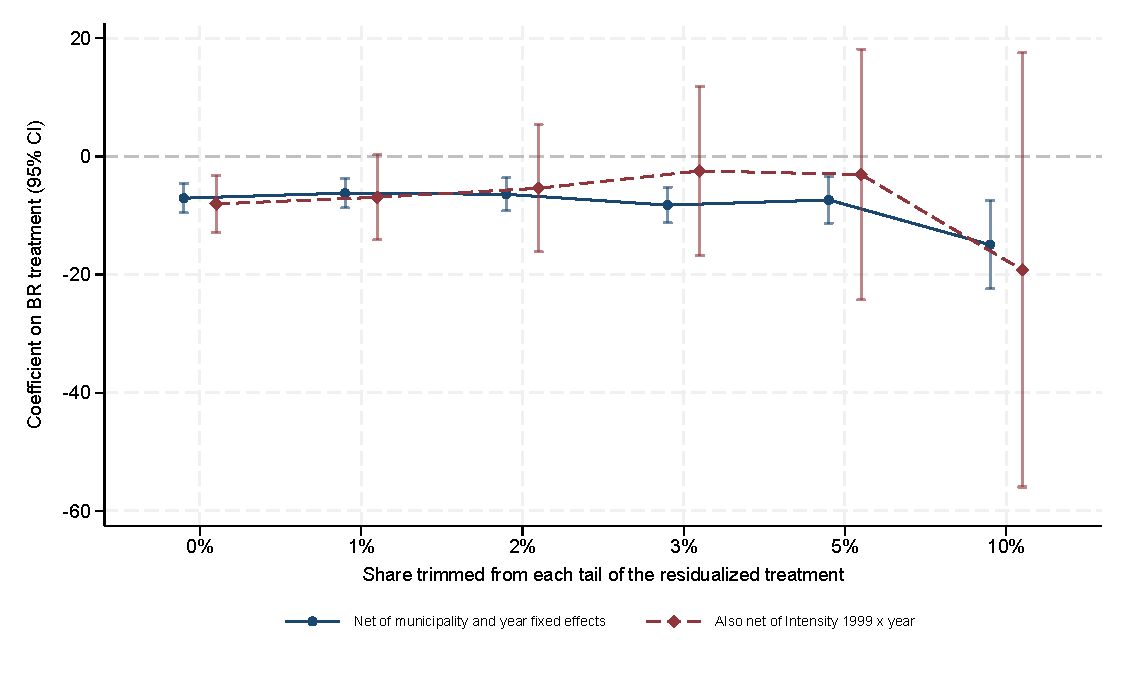
\includegraphics[width=0.49\textwidth]{figures/appendix/AF_br_trim_uw.pdf}}
    \subfigure[Weighted by population aged 65 and older]
     {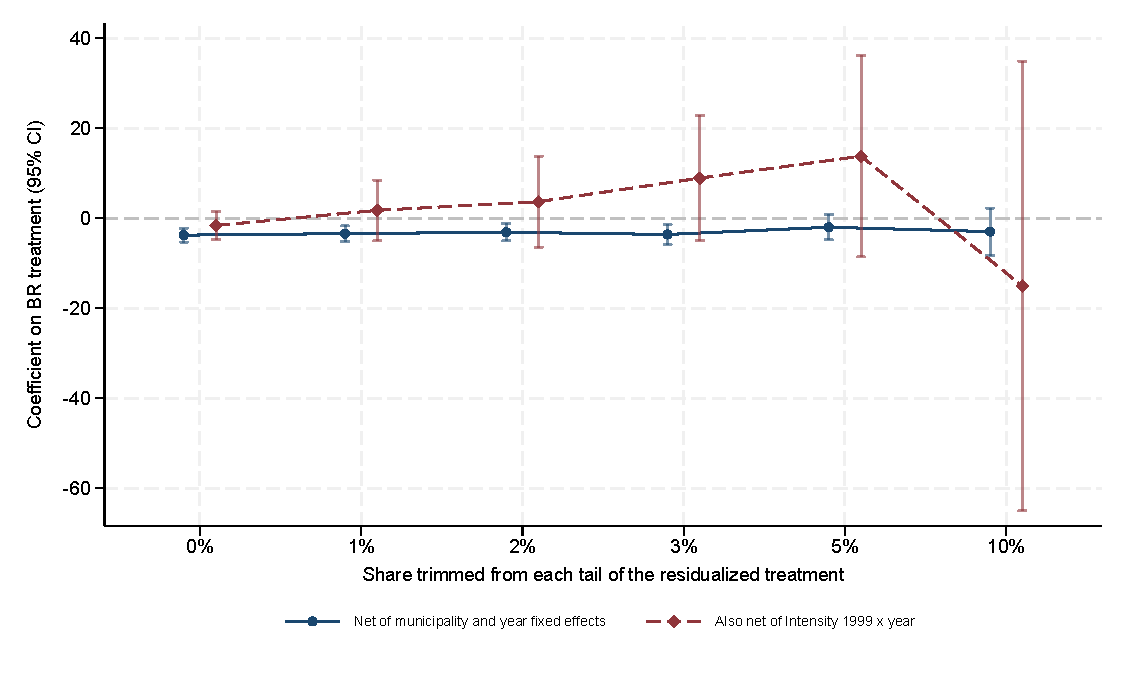
\includegraphics[width=0.49\textwidth]{figures/appendix/AF_br_trim_w.pdf}}

         \floatfoot{Notes: Each point is the coefficient on the treatment of \citet{BarhamRowberry2013JDE}, enrollment intensity lagged two years, in a regression of the mortality rate for adults aged 65 and older on that treatment and municipality and year fixed effects, in their sample (municipalities first incorporated in 1998 or 1999) and period (1992--2002); bars are 95\% confidence intervals with standard errors clustered at the municipality level. Moving right, the observations in the share of the sample shown are dropped from each tail of the treatment residualized on the fixed effects (circles) or on the fixed effects and $\textit{Intensity}_{1999}$ interacted with year indicators (diamonds), the variation our event study uses; each specification is trimmed on its own residualized treatment. The 0\% points reproduce the estimates in Appendix Table~\ref{at:br_leftover}, Panel~A. Stable coefficients indicate that the estimate does not hinge on a few extreme observations of the treatment.}
\end{figure}

\begin{figure}[H]
    \caption{Barham and Rowberry's Estimate by Municipality Size}
    \label{af:br_size}

    \subfigure[Unweighted]
     {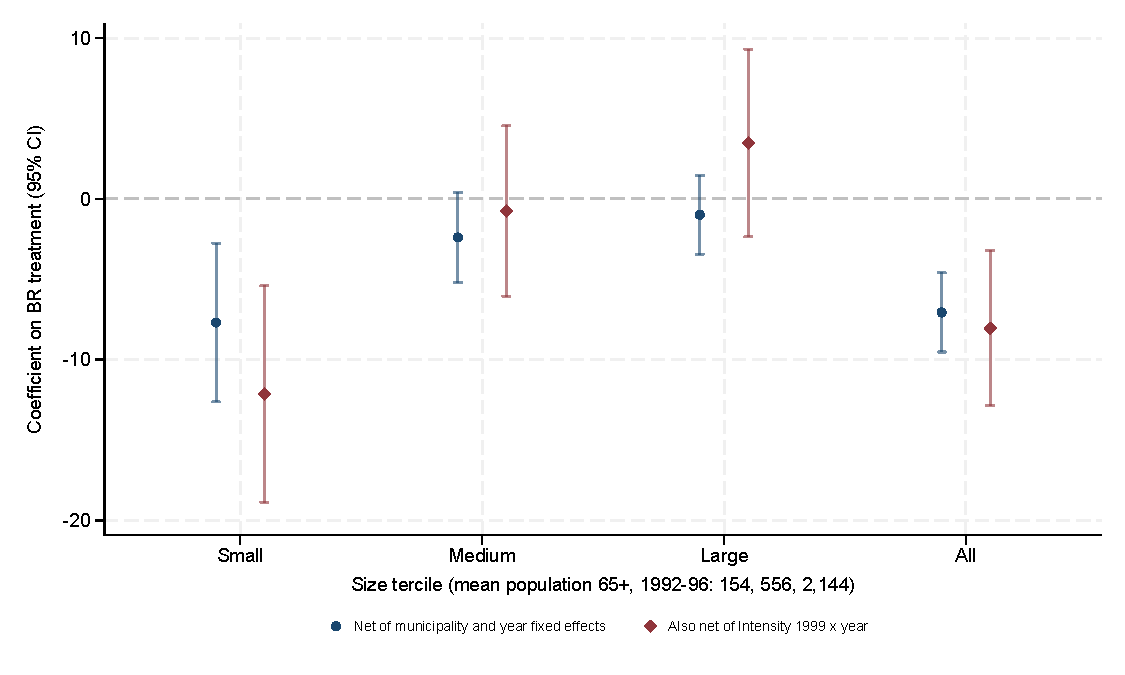
\includegraphics[width=0.49\textwidth]{figures/appendix/AF_br_size_uw.pdf}}
    \subfigure[Weighted by population aged 65 and older]
     {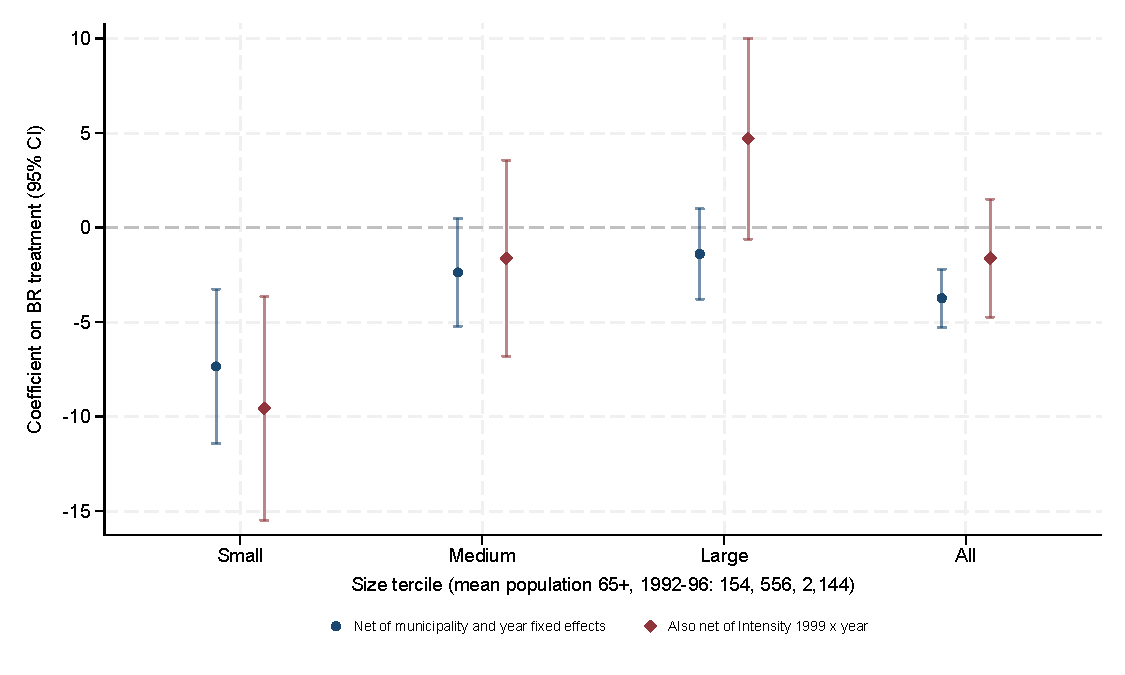
\includegraphics[width=0.49\textwidth]{figures/appendix/AF_br_size_w.pdf}}

         \floatfoot{Notes: Each point is the coefficient on the treatment of \citet{BarhamRowberry2013JDE}, enrollment intensity lagged two years, in a regression of the mortality rate for adults aged 65 and older on that treatment and municipality and year fixed effects, in their sample (municipalities first incorporated in 1998 or 1999) and period (1992--2002); bars are 95\% confidence intervals with standard errors clustered at the municipality level. Small, medium, and large are terciles of municipalities by their 1992--1996 average population aged 65 and older, with the tercile means given in the axis title; ``All'' is the full sample. Circles use the fixed effects only; diamonds also net out $\textit{Intensity}_{1999}$ interacted with year indicators, the variation our event study uses. Panel~(b) weights by population aged 65 and older within each sample. Small municipalities have noisy mortality rates, so a pattern that differs sharply across terciles would suggest that the pooled estimate partly reflects mortality-rate noise.}
\end{figure}

\begin{figure}[H]
    \caption{Event Study of the Variation in Barham and Rowberry's Treatment Not Explained by Intensity in 1999}
    \label{af:br_timing}

    \subfigure[Unweighted]
     {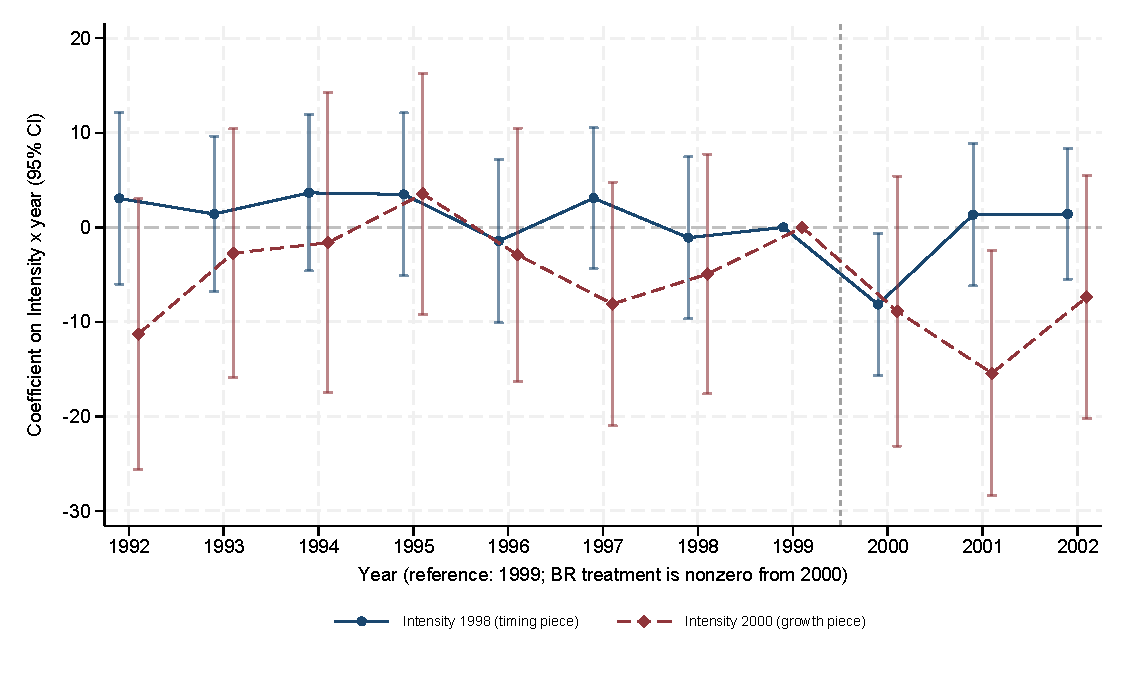
\includegraphics[width=0.49\textwidth]{figures/appendix/AF_br_timing_uw.pdf}}
    \subfigure[Weighted by population aged 65 and older]
     {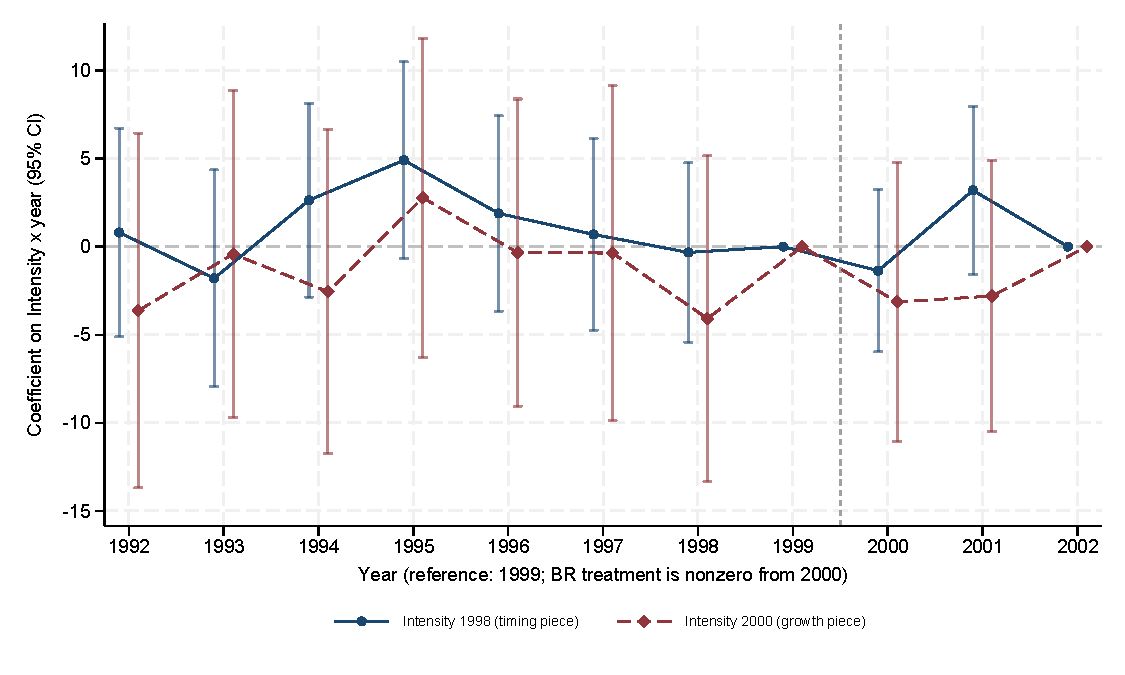
\includegraphics[width=0.49\textwidth]{figures/appendix/AF_br_timing_w.pdf}}

         \floatfoot{Notes: In the sample (municipalities first incorporated in 1998 or 1999) and period (1992--2002) of \citet{BarhamRowberry2013JDE}, their treatment, enrollment intensity lagged two years, is zero through 1999 and equals $\textit{Intensity}_{1998}$, $\textit{Intensity}_{1999}$, and $\textit{Intensity}_{2000}$ in 2000, 2001, and 2002. $\textit{Intensity}_{1999}$ interacted with year indicators therefore absorbs 2001 exactly, and what remains of their treatment is the 2000 value (the timing of enrollment before 1999, relevant because 1999 entrants have none) and the 2002 value (growth in enrollment after 1999). Each series comes from a regression of the mortality rate for adults aged 65 and older on municipality and year fixed effects, $\textit{Intensity}_{1999}$ interacted with year indicators, and the intensity shown interacted with year indicators, with 1999 as the reference year; points are the coefficients on the latter and bars are 95\% confidence intervals with standard errors clustered at the municipality level. The two intensities are entered in separate regressions. Coefficients for 1992--1998 are placebos: their treatment is zero in those years. The dashed vertical line marks the first year in which their treatment is nonzero. A coefficient for 2000 on $\textit{Intensity}_{1998}$ that is not preceded by similar coefficients in earlier years is the variation behind the estimate of \citet{BarhamRowberry2013JDE} that our design does not use; a drift in earlier years would instead indicate differential pre-trends.}
\end{figure}
